% Copyright (c) 2005-2008 Center for Urban Simulation and Policy Analysis,
% University of Washington.  Permission is granted to copy, distribute and/or
% modify this document under the terms of the GNU Free Documentation License,
% Version 1.2 or any later version published by the Free Software Foundation;
% with no Invariant Sections, no Front-Cover Texts, and no Back-Cover Texts.
% A copy of the license is included in the section entitled "GNU Free
% Documentation License".

\chapter{Interactive Exploration of Opus and UrbanSim}
\label{urbansim-tutorial}

\index{tutorial!\package{urbansim}}
This chapter gives a tutorial on using \package{opus_core} and \package{urbansim} in an interactive mode.
Running Python \pythonindex interactively provides a convenient way for both beginners
and experienced users to experiment with features and try out code.  This
tutorial is directed mainly to modelers, developers and other Opus users
who will experiment with single components of the package and develop new
features, rather than use the system of models as whole.

If necessary, install the supporting software, install Opus, and test
the installation, as described in Appendix~\ref{appendix:installation}.

You can start a Python session by opening a command window and
typing \verb|python| at the command prompt. Alternatively, the
Wing IDE \wingindex also provides a convenient Python shell window.

Any code after the \verb|>>>| is Python code.  To follow along with this
tutorial, enter this directly into a Python interpreter.  If you are unfamiliar
with Python, read Troubleshooting Python,
Section~\ref{sec:troubleshooting-python}, at the end of this chapter before
proceeding through the code.

\section{Working with Data Sets}
\label{sec:datasets}

A dataset \datasetindex in Opus is considered as a $n \times m$ table where $n$ is the
number of entries and $m$ is the number of characteristics, \characteristicsindex also called
attributes. \attributesindex One of the characteristics \characteristicsindex must have unique values
that are numeric larger than 0.

Suppose you have a set of household agents \index{household agents} with two characteristics, \characteristicsindex income
and number of persons per household, which are uniquely identified by
household IDs. The file \file{data/tutorial/households.tab} in the \package{urbansim}
package contains an example dataset \datasetindex for 10 households:
\begin{verbatim}
household_id   income         persons
 1               1000           2
 2               2000           3
 3               5000           3
 4               3000           2
 5                500           1
 6              10000           4
 7               8000           4
 8               1000           1
 9               3000           2
10              15000           5
\end{verbatim}

In Opus datasets are independent from the physical storage of the data. A data storage
is represented by a python object. We create a storage object for the ASCII file \file{households.tab}:

 \label{storagepage}
\begin{verbatim}
>>> import os
>>> import urbansim
>>> us_path = urbansim.__path__[0]
>>> from opus_core.storage_factory import StorageFactory
>>> storage = StorageFactory().get_storage('tab_storage',
        storage_location = os.path.join(us_path, 'data/tutorial'))
\end{verbatim}

\index{Storage!tab}
The \verb|storage| here specifies that the data
are stored as an ASCII file in a table format. 
Opus can support many types of storage formats, including formats you define. See Section~\ref{sec:data-storage}
for more details.

Now we create a household dataset \datasetindex with the \package{opus_core} class \class{Dataset} 
(see Section~\ref{sec:opus-core-datasets}), using the created
storage object:
\begin{verbatim}
>>> from opus_core.datasets.dataset import Dataset
>>> households = Dataset(in_storage = storage,
                         in_table_name = 'households', 
                         id_name='household_id',
                         dataset_name='household')
\end{verbatim}

\class{Dataset} supports lazy loading. Thus, there are no entries
loaded for \verb|households| at this moment:
\begin{verbatim}
>>> households.get_attribute_names()
[]
\end{verbatim}
But the dataset \datasetindex `knows' about attributes \attributesindex living on the given storage:
\begin{verbatim}
>>> households.get_primary_attribute_names()
['household_id', 'income', 'persons']
\end{verbatim}
The data are loaded as they are needed. For example, loading the
unique identifier of the dataset \datasetindex gives:
\begin{verbatim}
>>> households.get_id_attribute()
array([ 1,  2,  3,  4,  5,  6,  7,  8,  9, 10])
>>> households.size()
10
\end{verbatim}

Other attributes \attributesindex can be loaded via the \method{get_attribute()} \attributesindex method which
returns a numpy array:
\begin{verbatim}
>>> households.get_attribute("income")
array([  1000.,   2000.,   5000.,   3000.,    500.,  10000.,   8000.,
         1000.,   3000.,  15000.])
>>> households.get_attribute_names()
['household_id', 'income']
\end{verbatim}

Each attribute \attributesindex of a \class{Dataset} is stored as a numpy array. \numpyindex

In the above example, each of the attributes \attributesindex is
loaded separately. Alternatively, we can load multiple attributes
\attributesindex at once, which can be useful when loading data from
a slow storage, such as a SQL database:
\begin{verbatim}
>>> households.load_dataset()
>>> households.get_attribute_names()
['household_id', 'persons', 'income']
\end{verbatim}
An optional argument \verb|attributes| can be passed to the \method{load_dataset()}
method that specifies names of attributes \attributesindex to be loaded, e.g. \verb|attributes=['income', 'persons']|.

% The character "'" does comes out as a right-single-quote, not a vertical-
% quote, which makes it fail when copy-pasting from Acrobat to a Python shell.
% Is there any way to force this to be a vertical quote?

% (terhorst) The answer is, "Yes." There's a handy little macro called
% "upquote" that does exactly this for \verbatim and \verb.

We can also plot a histogram \histogramindex of the income attribute \attributesindex (this method requires the
  \module{matplotlib} \matplotlibindex library):

\histogramindex
\begin{verbatim}
>>> households.plot_histogram("income", bins = 10)
\end{verbatim}
\begin{center}
%begin{latexonly}
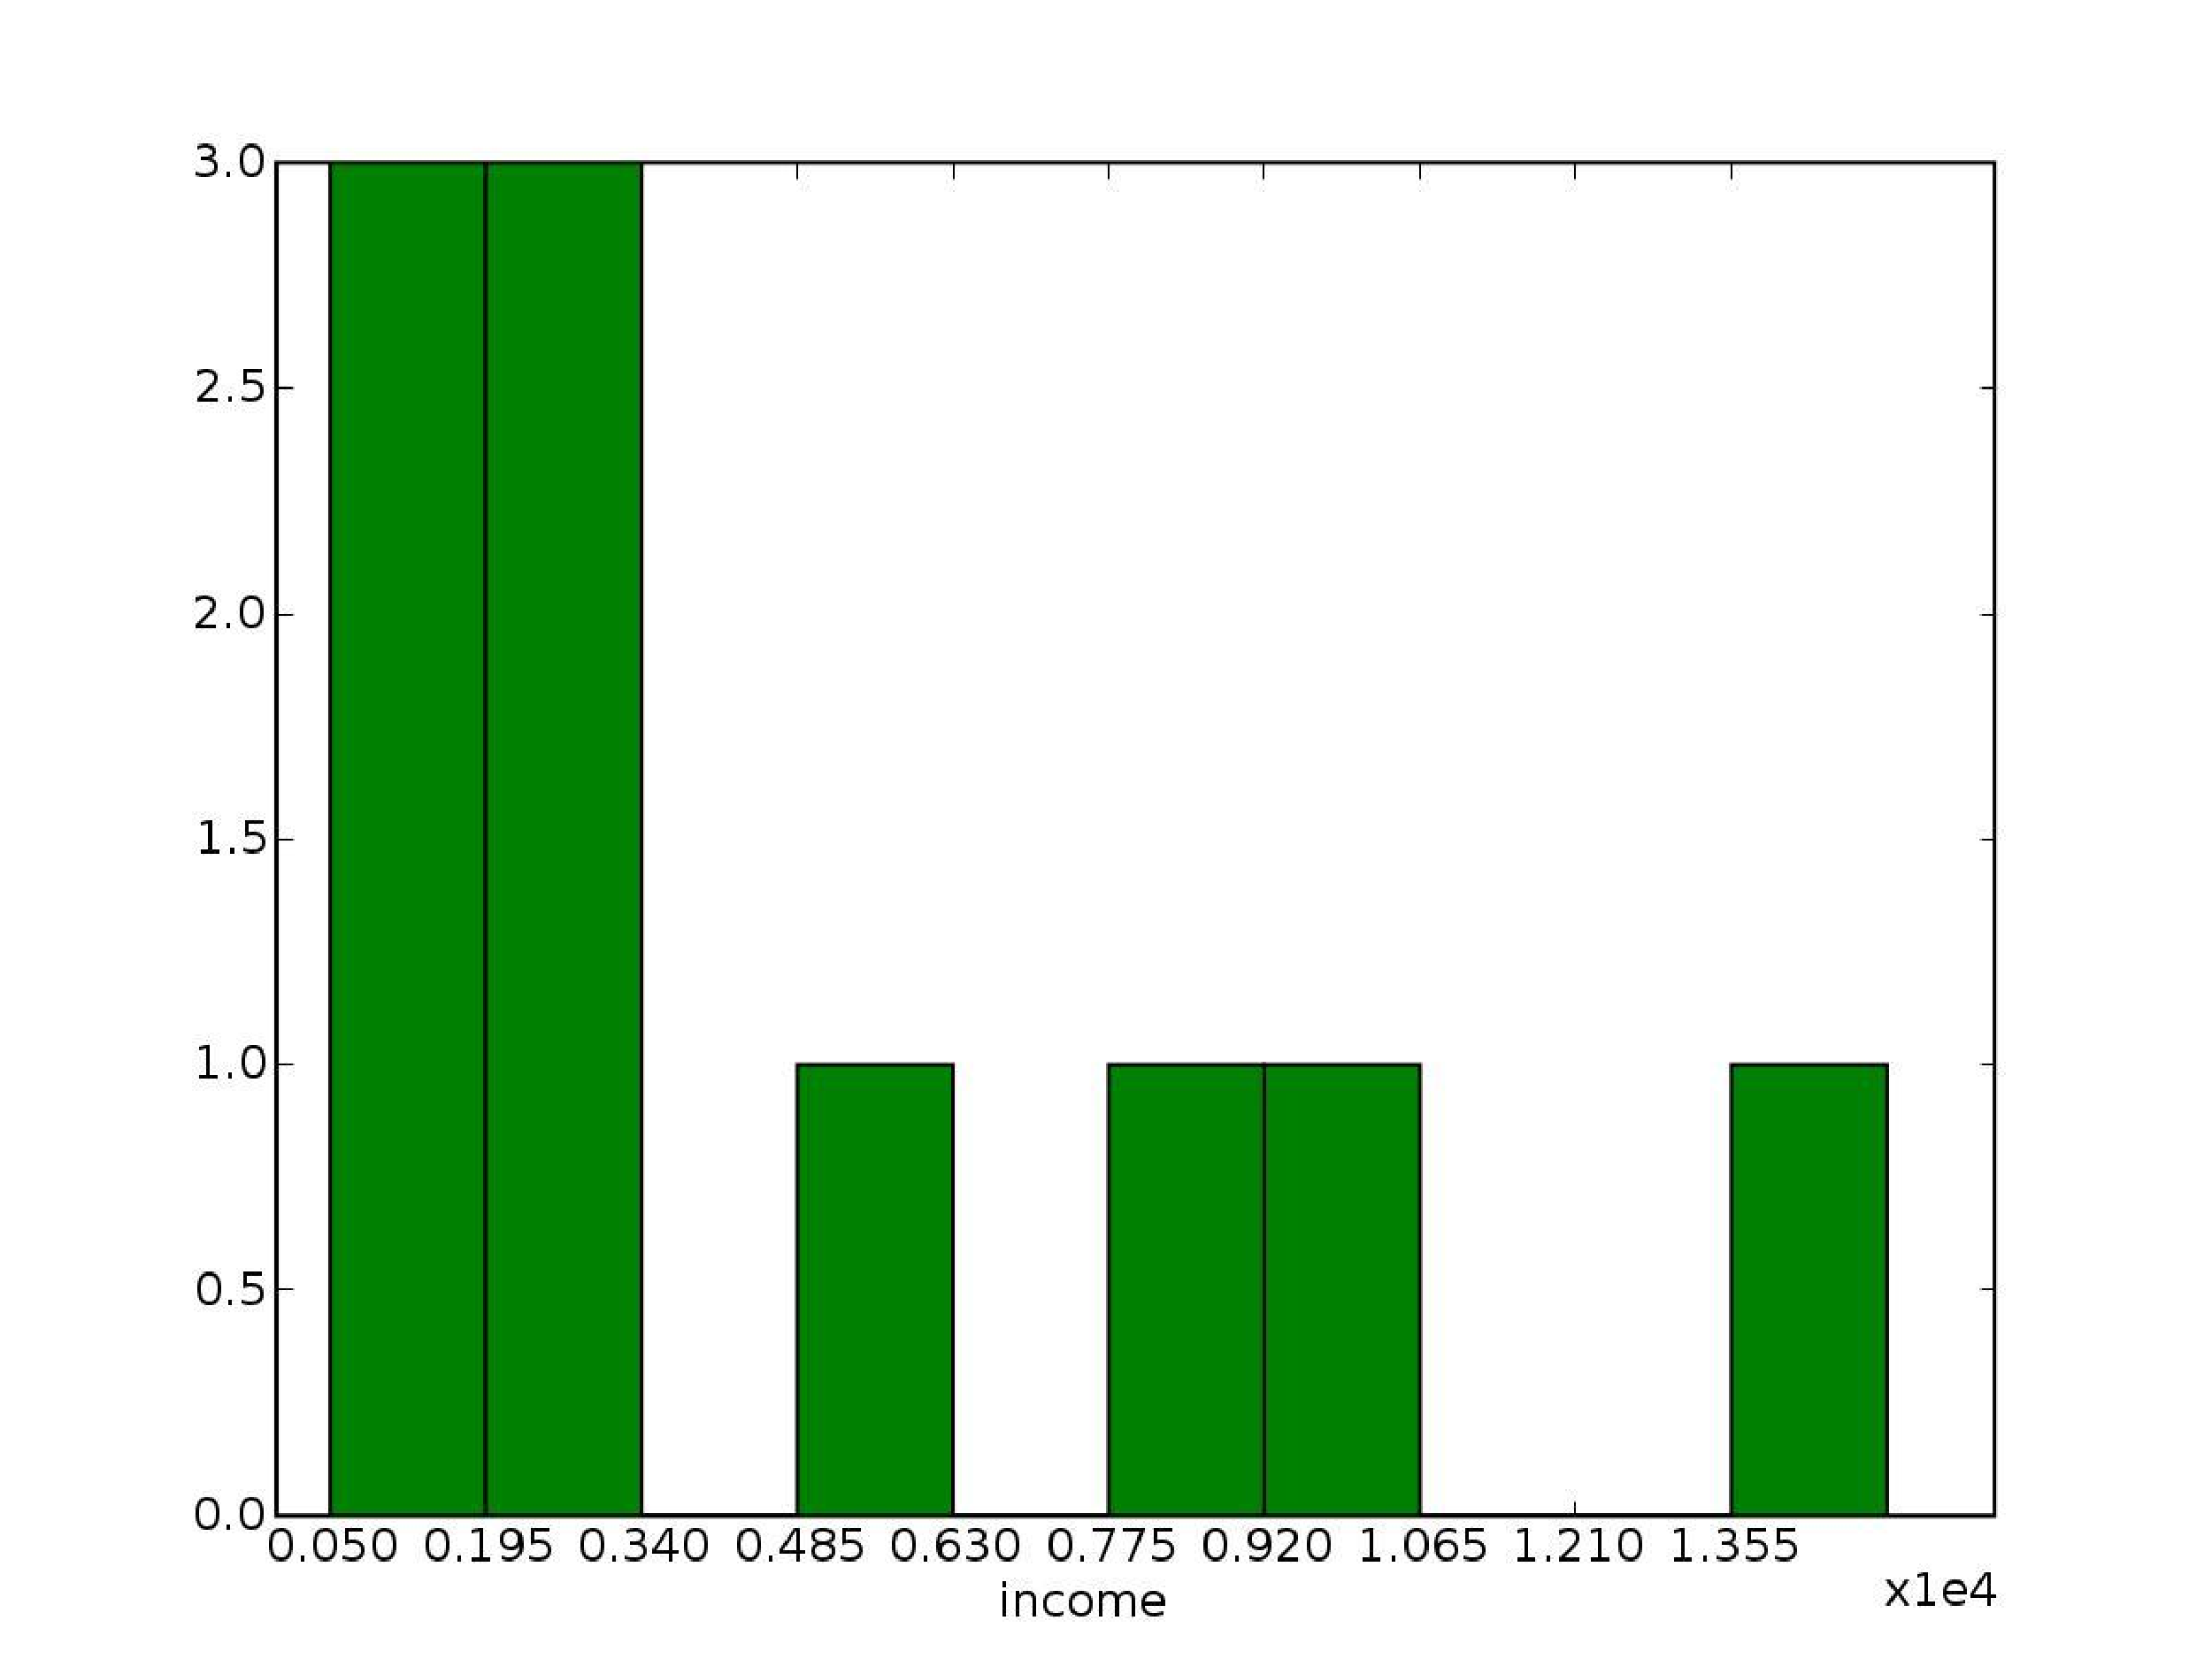
\includegraphics[scale=0.2, angle=0]{images/incomehist.pdf}
%end{latexonly}
\htmlonly{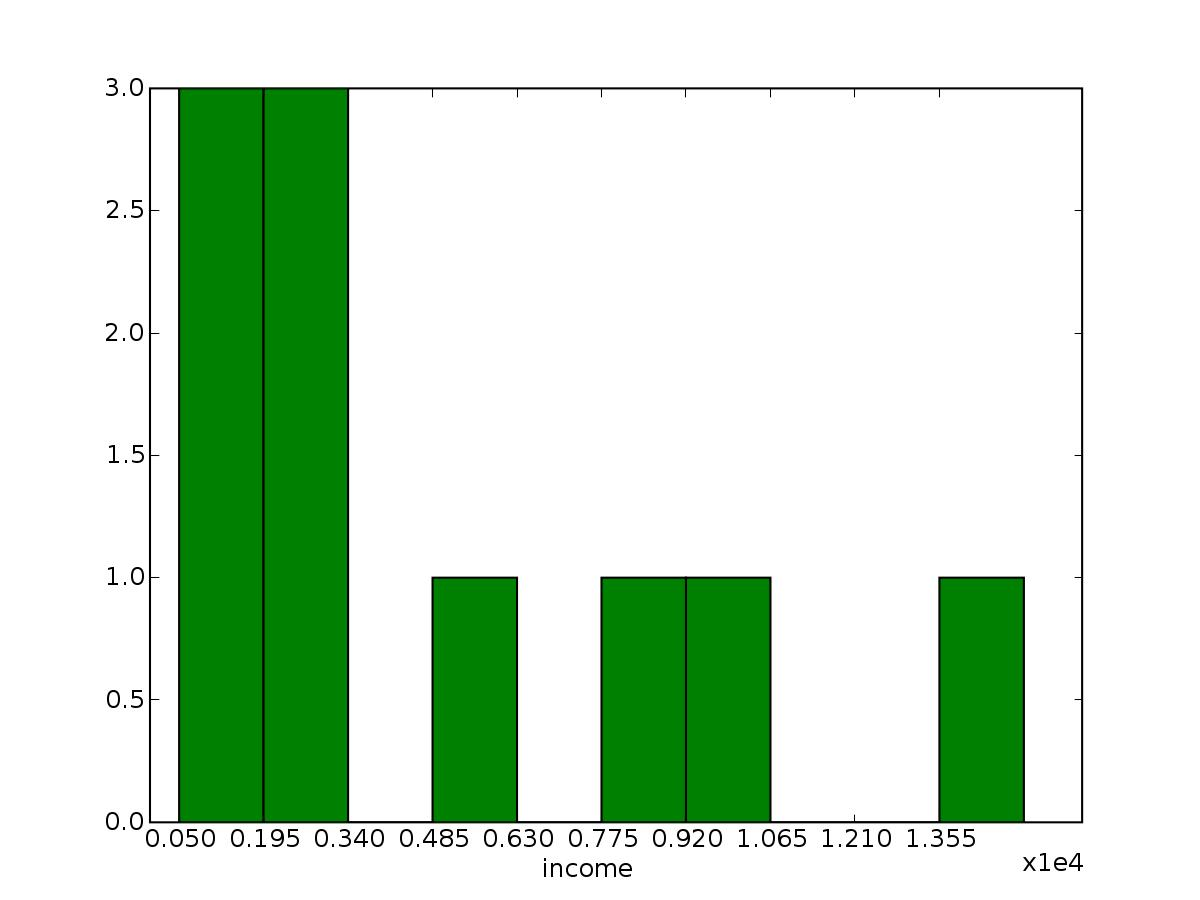
\includegraphics[scale=0.6, angle=0]{images/incomehist.jpg}}
\end{center}
or (if the \module{rpy} \rpyindex library is installed)
\histogramindex
\begin{verbatim}
>>> households.r_histogram("income")
\end{verbatim}
\begin{center}
%begin{latexonly}
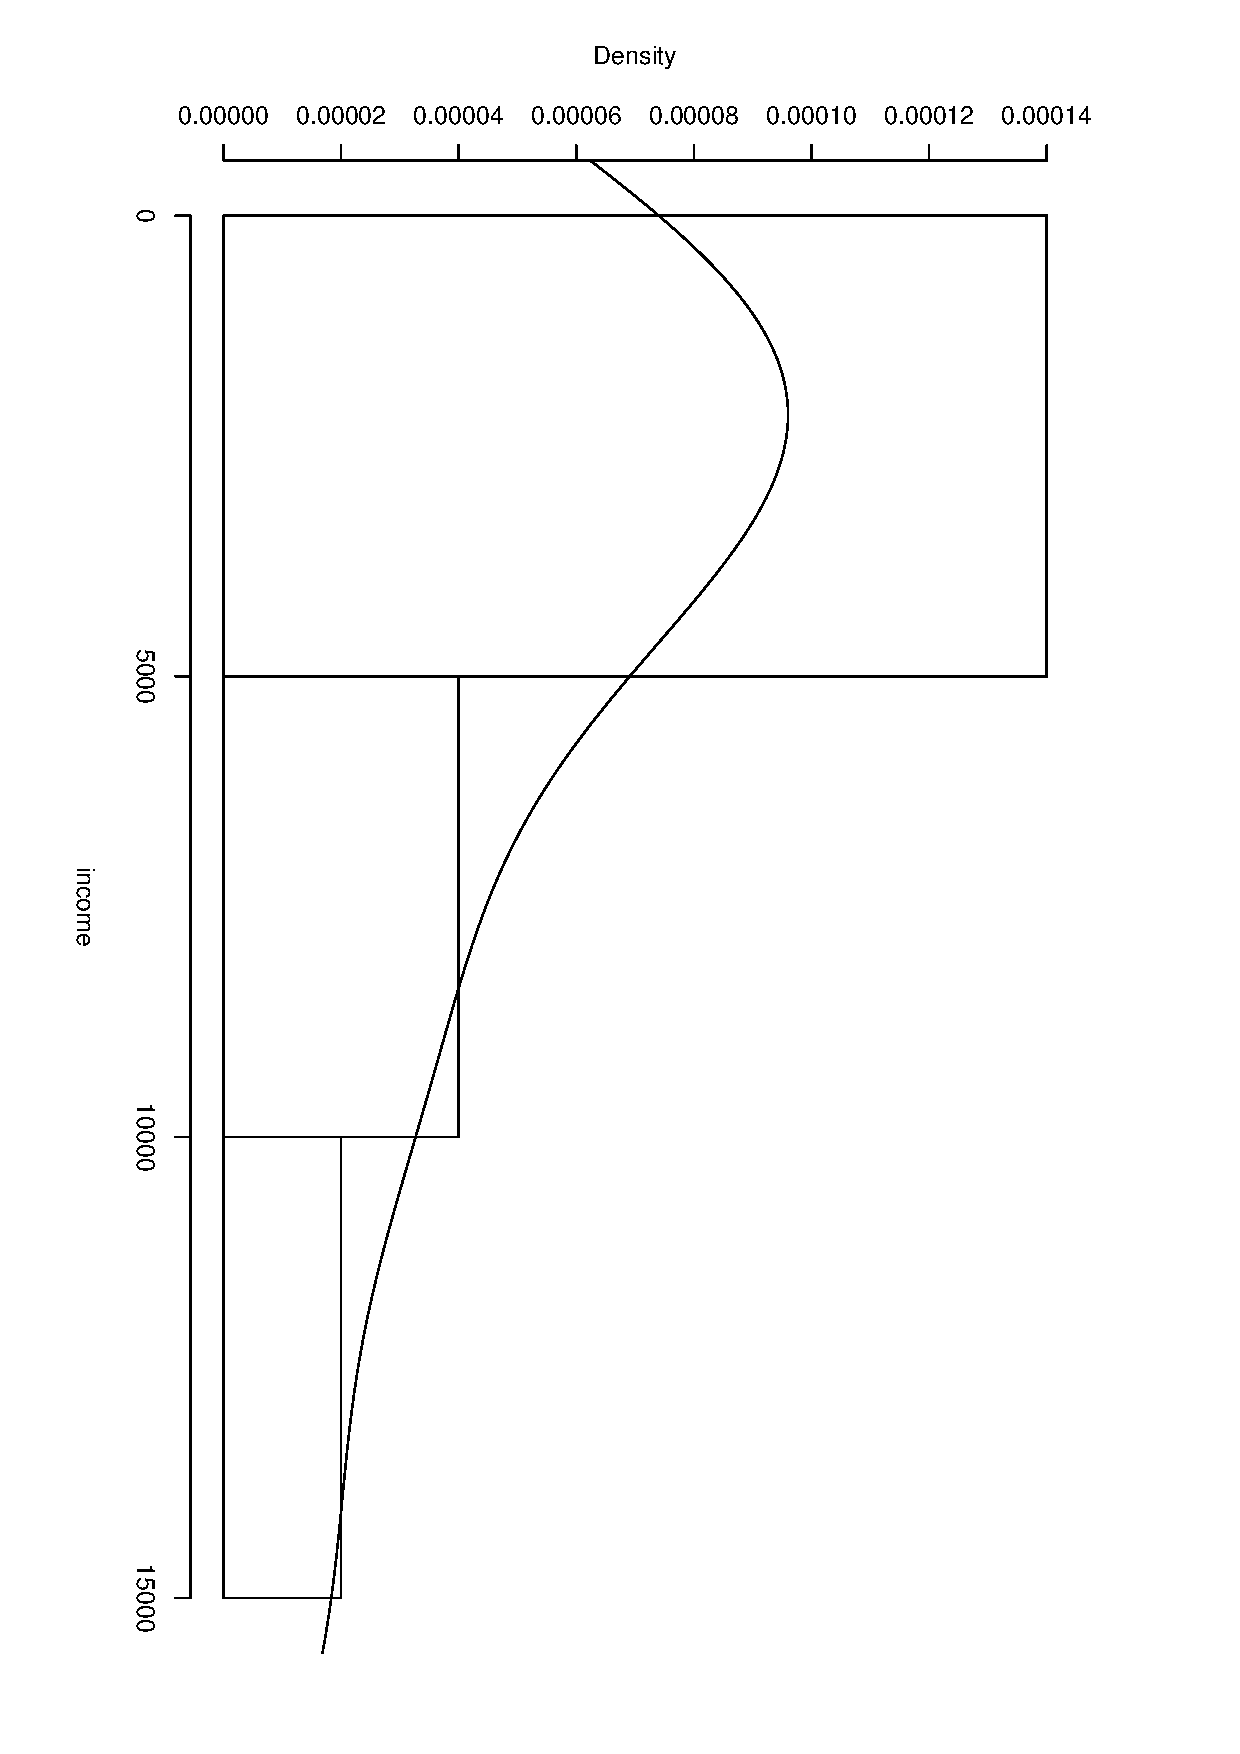
\includegraphics[scale=0.3, angle=90]{images/incomerhist.pdf}
%end{latexonly}
\htmlonly{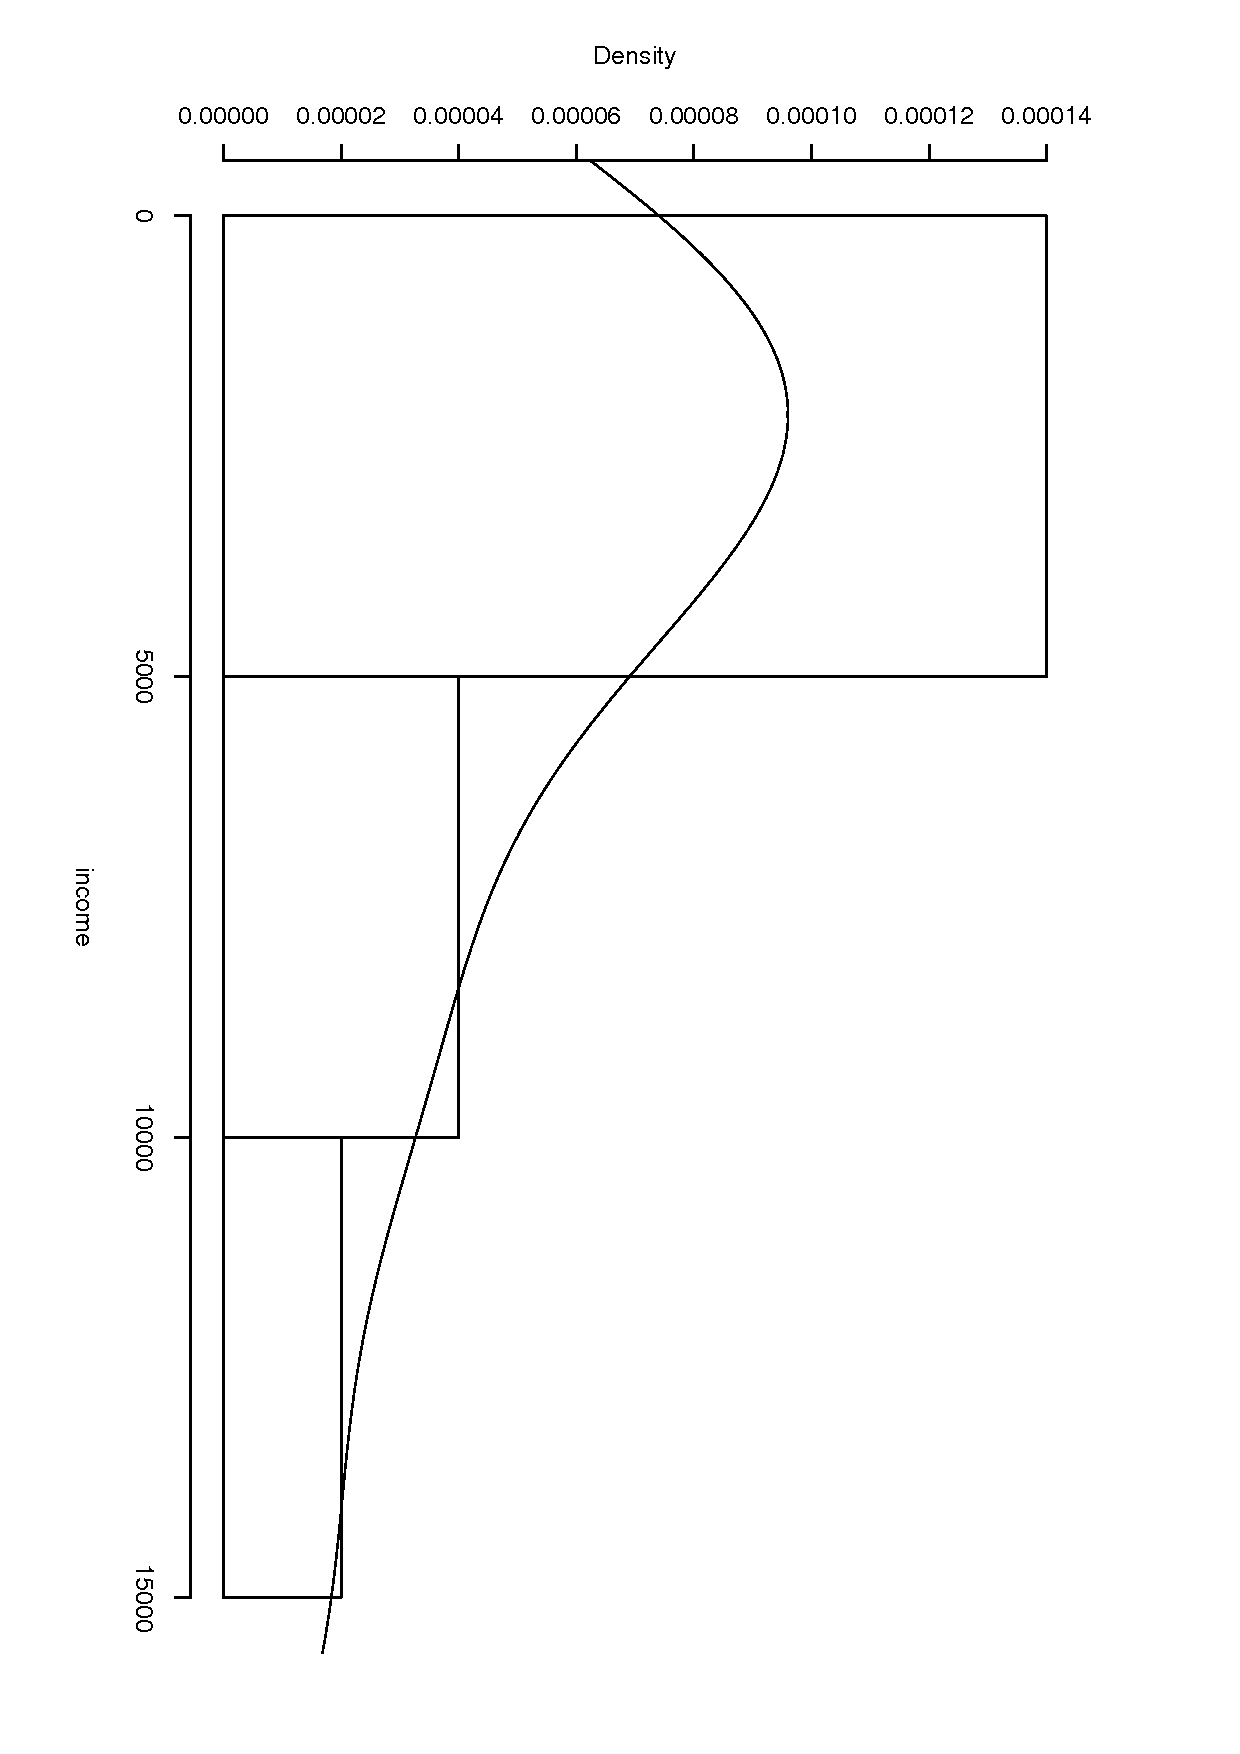
\includegraphics[scale=0.3, angle=90]{images/incomerhist.jpg}}
\end{center}

We can investigate a correlation \index{correlation} between attributes \attributesindex by plotting a scatter
plot \scatterplotindex (\module{rpy} \rpyindex library required):
\scatterplotindex
\begin{verbatim}
>>> households.r_scatter("persons", "income")
\end{verbatim}
\begin{center}
%begin{latexonly}
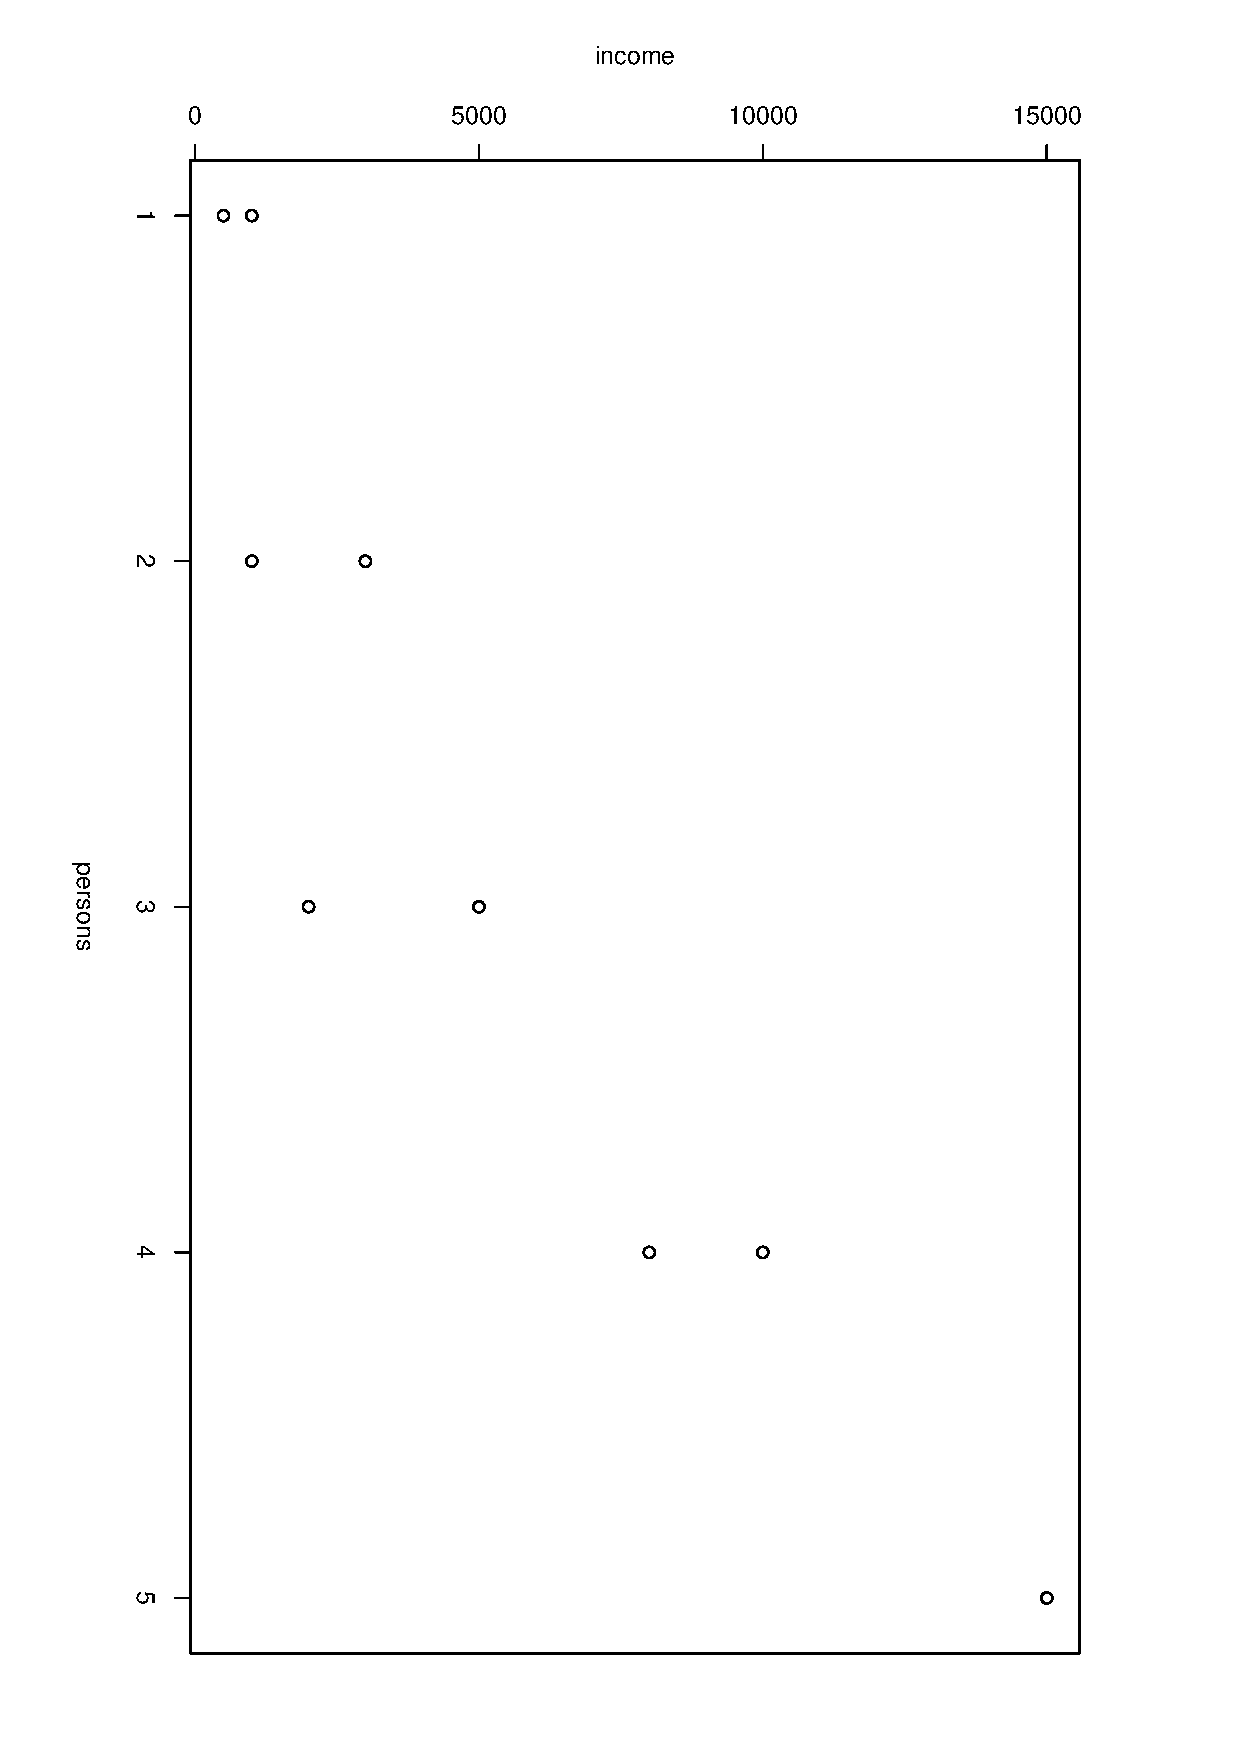
\includegraphics[scale=0.3, angle=90]{images/incomerscatter.pdf}
%end{latexonly}
\htmlonly{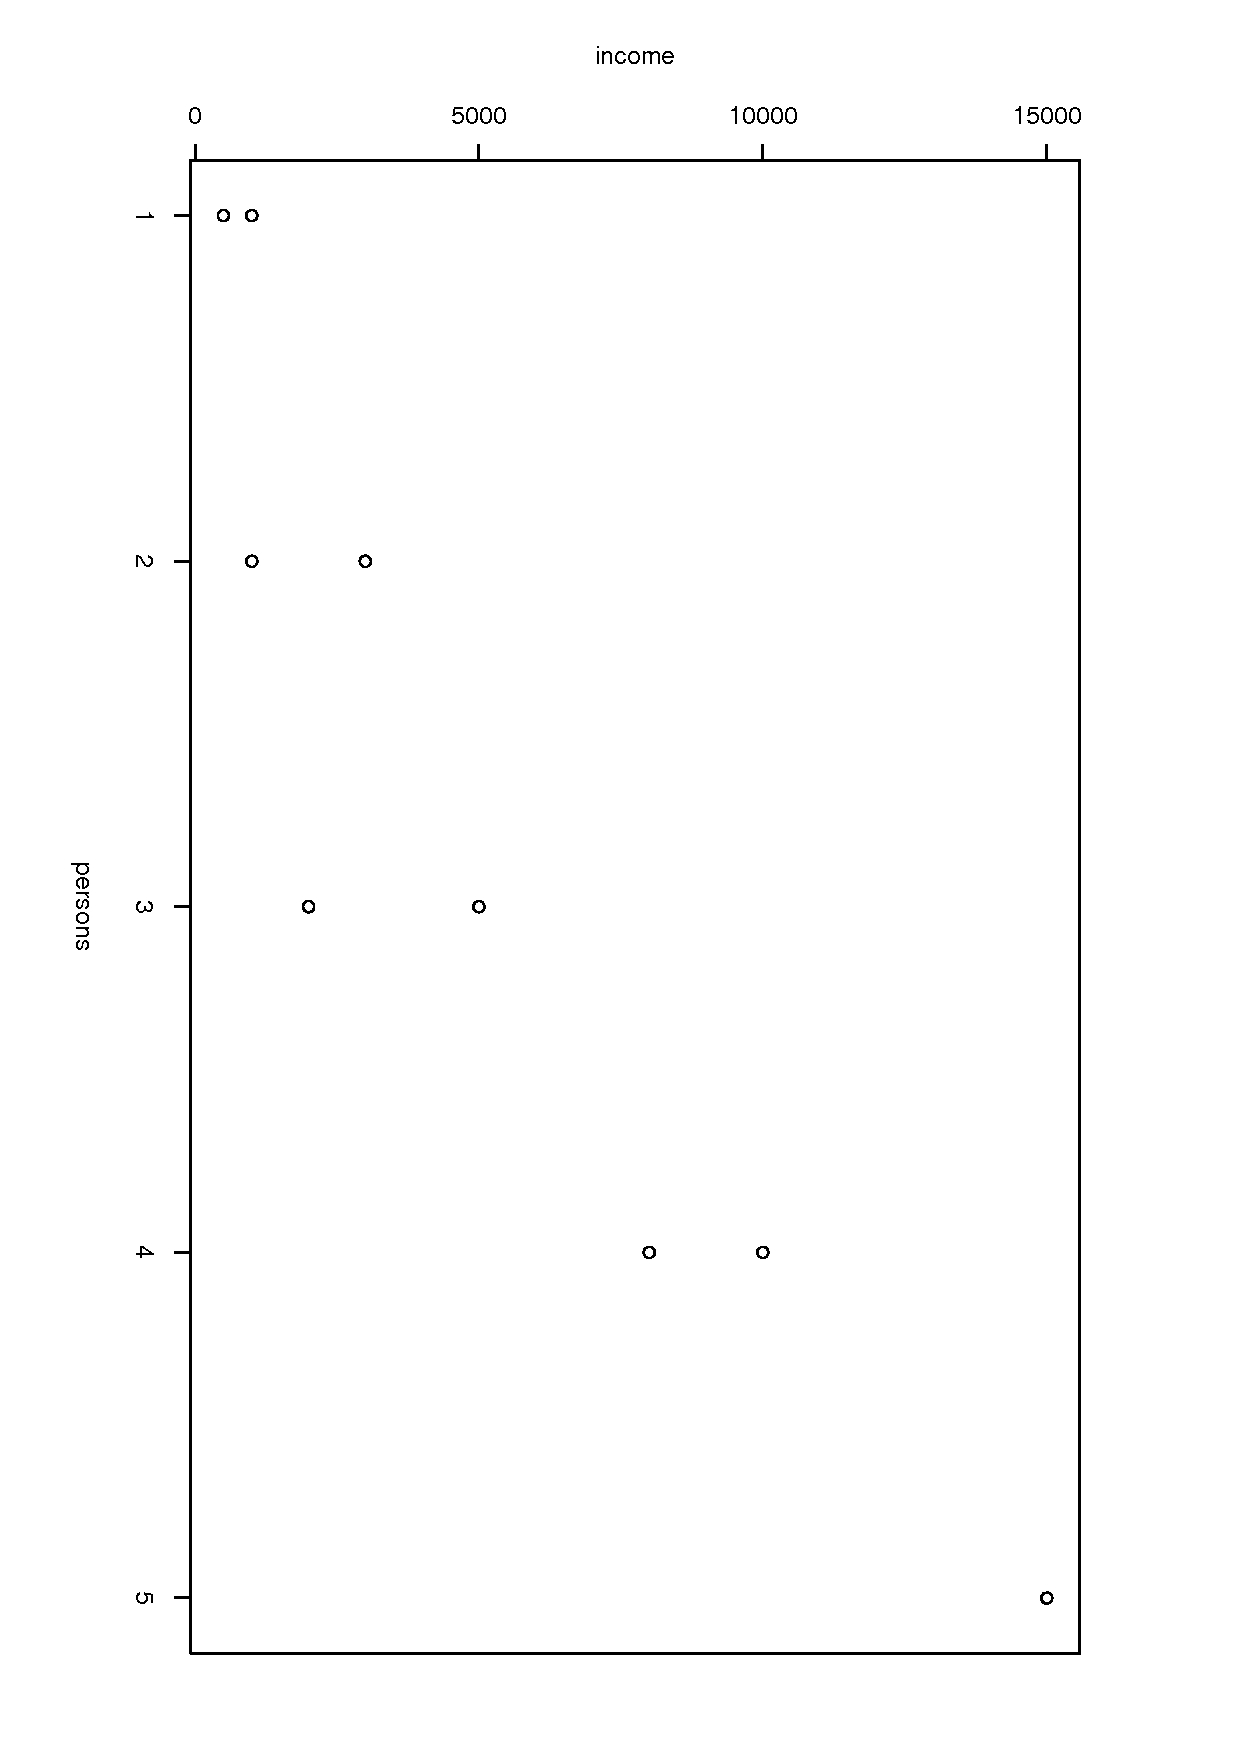
\includegraphics[scale=0.3, angle=90]{images/incomerscatter.jpg}}
\end{center}
\coefficientsindex
\begin{verbatim}
Correlation coefficient:  0.919147133827
\end{verbatim}

The correlation coefficient between two attributes and the correlation matrix of several attributes, respectively,
can be obtained by:
\begin{verbatim}
>>> households.correlation_coefficient("persons", "income")
0.91914713382720947
>>> households.correlation_matrix(["persons", "income"])
array([[ 1.        ,  0.91914713],
       [ 0.91914713,  1.        ]], type=float32)
\end{verbatim}

A summary of data in a dataset \datasetindex can by given by:

\attributesindex
\begin{verbatim}
>>> households.summary()
Attribute name        mean           sd           sum        min     max
-------------------------------------------------------------------------
       persons         2.7         1.34            27          1       5
        income      4850.0      4749.56         48500        500   15000
       


Size: 10  records
identifiers:
        household_id  in range  1 - 10
\end{verbatim}

To add an attribute \attributesindex to the set of households, for example each
household's location, we do
\begin{verbatim}
>>> households.add_primary_attribute(data=[4,6,9,2,4,8,2,1,3,2], name="location")
>>> households.get_attribute_names()
['household_id', 'persons', 'location', 'income']
\end{verbatim}
If the attribute \attributesindex "location" already exists in the dataset, \datasetindex the values are
overwritten.

To change specific values in a dataset, \datasetindex one can use

\attributesindex
\begin{verbatim}
>>> households.modify_attribute(name="location", data=[0,0], index=[0,1])
>>> households.get_attribute("location")
array([0, 0, 9, 2, 4, 8, 2, 1, 3, 2])
\end{verbatim}
Here the argument \verb|index| determines the index of the data that are
modified.

To determine the location of household with \verb|household_id| $= 5$,
do
\begin{verbatim}
>>> households.get_data_element_by_id(5).location
4
\end{verbatim}

In order to store data in one of the supported formats,
you can use the {\tt storage} object created at the beginning of this section, or create a new one using
a different type of storage:

\datasetindex
\begin{verbatim}
>>> households.write_dataset(out_storage=storage,
                             out_table_name="households_output")
\end{verbatim}

Each dataset \datasetindex
  should have a unique dataset \datasetindex name that is used as an identification in
  variable \variablesindex computation (see
  Section~\ref{sec:variable-names}). 

\begin{verbatim}
>>> households.get_dataset_name()
'household'
\end{verbatim}

The \package{urbansim} package contains many pre-defined dataset \datasetindex classes, such as \class{HouseholdDataset}, \class{GridcellDataset},
  \class{JobDataset}, \class{ZoneDataset}, \class{FazDataset}, \class{NeighborhoodDataset}, \class{RaceDataset},
  \class{RateDataset}. Some datasets are described in  Section~\ref{sec:urbansim-datasets},
  Table~\ref{tab:urbansim-datasets}. They are all children of \class{Dataset} with pre-defined values
  for some arguments, such as \verb|id_name|, \verb|in_table_name| or \verb|dataset_name|. 

  

%
\section{Working with Models}
%
Generally, each model class has a method \method{run()} that runs a simulation and
(if applicable) a method \method{estimate()} that runs an estimation of the model.
Models are initiated by a constructor that sets class attributes common to
both methods.

%
\subsection{Choice Model}
%
The class \class{ChoiceModel} implemented in \package{opus_core} is initiated with a choice set
and a set of components specifying some of the model behavior. The model can
be estimated and run for a set of agents (see Section~\ref{sec:choice-model} for details).

%
\subsubsection{Initialization}
%
Suppose we would like to simulate a process of households deciding among 3
choices using the discrete choice model theory. The number of persons in each
household should influence their decisions. We will model this behavior by
multinomial logit using a system of utility functions:
$$
\begin{array}{rcrr}
v_1 & = &\beta_{01} & \\
v_2 & = &  & \beta_{12}x \\
v_3 & = & \beta_{03} & +  \beta_{13}x
\end{array}
$$
Here, $\beta_{01}$ and $\beta_{03}$ are alternative specific constants and $x$
is a household variable \variablesindex ``persons''.

The model is initialized by
\begin{verbatim}
>>> from opus_core.choice_model import ChoiceModel
>>> choicemodel = ChoiceModel(
                       choice_set=[1,2,3],
                       utilities = "opus_core.linear_utilities",
                       probabilities = "opus_core.mnl_probabilities",
                       choices = "opus_core.random_choices")
\end{verbatim}
Thus, the model is composed by external implementations of model steps, such
as computing utilities, computing probabilities and computing choices,
specified as \module{package.module_name}. Those modules must contain a
class of the same name and a method \method{run()} that performs the actual
computation (see Section~\ref{sec:choice-model} and Sections~\ref{sec:utilities}-\ref{sec:choices}
for more details).

%
\subsubsection{Estimation}
%
In order to estimate coefficients \coefficientsindex $\beta$ from the above equations, we define
a specification:

\coefficientsindex \variablesindex
\begin{verbatim}
>>> from numpy import array
>>> from opus_core.equation_specification import EquationSpecification
>>> specification = EquationSpecification(
      coefficients = array([
        "beta01",      "beta12",         "beta03",    "beta13"
                          ]),
      variables = array([
        "constant","household.persons", "constant", "household.persons"
                        ]),
      equations = array([
           1,              2,                3,             3
                    ])
      )
\end{verbatim}
Each of the arguments is an array where the $i$th element describes the $i$th
coefficient \coefficientsindex in an equation determined by the $i$th element in the argument
\verb|equations|. For example, \verb|beta12| is a coefficient \coefficientsindex connected to the
household variable \variablesindex ``persons'' in equation 2, and \verb|beta03| is a constant
used in equation 3. The prefix ``household'' in the variable \variablesindex name specifies
the name of the dataset \datasetindex \verb|households|.
In other words, we are using here a dataset-qualified \datasetindex name of an attribute \attributesindex explained in
Section~\ref{sec:opus-core-attribute-names}.
An optional argument \verb|submodels| can extend the specification
to a model with multiple submodels. The \class{EquationSpecification} class is described
in Section~\ref{sec:specification} in more detail.

Our estimation data must include an attribute \attributesindex specifying choices that
households made:
\begin{verbatim}
>>> households.add_primary_attribute(data=[1,2,2,2,1,3,3,1,2,1], name="choice_id")
\end{verbatim}

The estimation is done by passing the specification, the agent set for
estimation and a name of the module that implements the actual estimation to
the method \method{estimate()}:
\coefficientsindex
\begin{verbatim}
>>> coefficients, other_results = choicemodel.estimate(
                         specification, households, 
                         procedure="opus_core.bhhh_mnl_estimation")
\end{verbatim}
\begin{verbatim}
Estimating Choice Model (from opus_core.choice_model): started on 
                                                    Wed Nov  5 12:04:17 2008
    submodel: -2
    Convergence achieved.
    Akaike's Information Criterion (AIC):  26.142396805
    Number of Iterations:  144
    ***********************************************
    Log-likelihood is:            -9.07119840248
    Null Log-likelihood is:       -10.9861228867
    Likelihood ratio index:       0.174303938155
    Adj. likelihood ratio index:  -0.189791752496
    Number of observations:       10
    Suggested |t-value| >         1.51742712939
    Convergence statistic is:     0.000990037670084
    -----------------------------------------------
    Coeff_names	estimate	std err		t-values
        beta01	0.432678	 3.14438	0.137604
        beta03	-4.51824	 21.7087	-0.208131
        beta12	0.180115	 1.72541	 0.10439
        beta13	 1.34052	 4.18176	0.320564
    ***********************************************
    Elapsed time:  0.064521 seconds
Estimating Choice Model (from opus_core.choice_model): completed.........0.1 sec

\end{verbatim}
The estimation module given in the argument \verb|procedure| is a child of
\class{EstimationProcedure} (see Section~\ref{sec:estimation-procedure}), must
contain a method \method{run()} and should return a dictionary with keys
''estimators'' and ``standard_errors'' respectively, that contain arrays of
the estimated values and their standard errors, respectively.  The \method{estimate()}
method returns a tuple where the first element is an instance of
class \class{Coefficients} \coefficientsindex and the second element is a dictionary with all
results returned by the estimation \verb|procedure|.

A coefficient \coefficientsindex object can
be stored in a storage. For example, to store the computed coefficients \coefficientsindex as an
ASCII file \file{mycoef.tab} in the directory defined in the \verb|storage| object
on page~\pageref{storagepage}, do
\coefficientsindex
\begin{verbatim}
>>> coefficients.write(out_storage=storage, out_table_name="mycoef")
\end{verbatim}
Again, other types of storage can be used here.

 %

\subsubsection{Simulation}
%
The coefficients \coefficientsindex that result from the estimation run can be directly plugged
into a simulation run:
\coefficientsindex
\begin{verbatim}
>>> choices = choicemodel.run(specification,  coefficients, households)
Running Choice Model (from opus_core.choice_model): 
                                            started on Wed Nov  5 12:10:20 2008
    Total number of individuals: 10
    ChoiceM chunk 1 out of 1.: started on Wed Nov  5 12:10:20 2008
        Number of agents in this chunk: 10
    ChoiceM chunk 1 out of 1.: completed.................................0.0 sec
Running Choice Model (from opus_core.choice_model): completed............0.0 sec
>>> choices
array([1, 2, 1, 2, 2, 3, 3, 1, 2, 3])
\end{verbatim}
The resulting \verb|choices| is an array specifying the choice for each household. We can
now assign those values to the dataset: \datasetindex
\begin{verbatim}
>>> households.modify_attribute(name="choice_id", data=choices)
\end{verbatim}

Note that multiple runs will produce different results, which is due to random
numbers \index{random numbers} used within the model. In order to receive reproducible results\index{reproducible results}, one
can fix the seed of the random number generator. The call above was
preceded by
\numpyindex
\begin{verbatim}
>>> from numpy.random import seed
>>> seed(1)
\end{verbatim}

For demonstration purposes, we use the same dataset of households
for estimation and simulation. This would not be usually the case in real
simulation runs.

We can also create a coefficient \coefficientsindex class and assign their values directly
(see Section~\ref{sec:coefficients} for more details):
\coefficientsindex
\begin{verbatim}
>>> from opus_core.coefficients import Coefficients
>>> coefficients = Coefficients(
                     names=array(["beta01", "beta12", "beta03", "beta13"]),
                     values=array([0.5,      0.2,       -5.0,     1.3]))
\end{verbatim}

If a variable \variablesindex $x$ in the utility equations is choice dependent,
one can create a dataset \datasetindex of choices and assign this attribute to the
dataset. \datasetindex Besides a list and an array, the argument \verb|choice_set| in the
\class{ChoiceModel} constructor also accepts a dataset. \datasetindex

%
\subsection{Location Choice Model}
%
\label{sec:LCM}
%
The \class{LocationChoiceModel} class implemented in \package{urbansim} is a special case of the
\class{ChoiceModel} class (see Section~\ref{sec:location-choice-model} for details).
The choice set is a set of locations that agents choose
from. A set of locations can be sampled to each agent.

Suppose that in addition to the set of 10 households, we have a set of 9
locations with the attributes cost of living and capacity, respectively,
stored in a file \file{locations.tab}:
\begin{verbatim}
location  cost  capacity
1        500    1
2        200    1
3        600    2
4       1000    3
5        100    1
6       2000    3
7        300    1
8        400    1
9        800    2
\end{verbatim}
One can represent this dataset using again the  \class{Dataset} class:
\label{page:tutorial-gc-locations}
\begin{verbatim}
>>> locations = Dataset(in_storage = storage,
                        in_table_name = 'locations', 
                        id_name='location',
                        dataset_name='gridcell')
\end{verbatim}
We use here the \verb|storage| object
created on page~\pageref{storagepage}, since the table is stored in the same directory.

Suppose, we wish to simulate a process of agents choosing locations.  As a
first example, suppose our only predictor is the location attribute cost with
a coefficient \coefficientsindex value of $-0.01$ (modeling a negative effect of cost on the
choice preferences). (For simplicity, we skip the estimation process and
consider the coefficient \coefficientsindex value as given.) As in the previous section, we
create a coefficient \coefficientsindex object, a specification object and a choice model object,
respectively:

\coefficientsindex \variablesindex
\begin{verbatim}
>>> coefficients = Coefficients(names=("costcoef", ), values=(-0.01,))
>>> specification = EquationSpecification(variables=("gridcell.cost", ),
                                          coefficients=("costcoef", ))
>>> from urbansim.models.household_location_choice_model import \
                               HouseholdLocationChoiceModel
>>> hlcm = HouseholdLocationChoiceModel(
                               location_set = locations,
                               sampler=None,
                               compute_capacity_flag=False)
\end{verbatim}
The household location choice model (HLCM) is a child of 
\class{LocationChoiceModel} with some useful default settings.  
The argument \verb|sampler| specifies a module to be
used for sampling locations to each agent. If it is None, all locations are
considered as a possible alternative for each agent.  The argument
\verb|compute_capacity_flag| specifies if the procedure should take capacity of
locations into account.

We can run the HLCM by using the method \method{run()}
which takes as obligatory arguments \verb|specification|, \verb|coefficients| \coefficientsindex
and the set of agents for which the model runs.  
\coefficientsindex
\begin{verbatim}
>>> seed(1)
>>> result = hlcm.run(specification, coefficients, agent_set=households)
Running Household Location Choice Model 
                 (from urbansim.models.household_location_choice_model): 
                                     started on Wed Nov  5 12:53:11 2008
    Total number of individuals: 10
    HLCM chunk 1 out of 1.: started on Wed Nov  5 12:53:11 2008
        Number of agents in this chunk: 10
    HLCM chunk 1 out of 1.: completed....................................0.0 sec
Running Household Location Choice Model 
      (from urbansim.models.household_location_choice_model): completed...0.0 sec

\end{verbatim}

The results of the HLCM run determine locations that
agents have chosen. The model modifies values of the attribute \attributesindex `location' of
the agent set or adds this attribute \attributesindex to the dataset, \datasetindex if it doesn't exist:
\attributesindex
\begin{verbatim}
>>> households.get_attribute("location")
array([5, 5, 5, 5, 5, 7, 7, 2, 5, 5])
\end{verbatim}

One way of visualizing results of the HLCM run is to plot a histogram \histogramindex of the
choices, including the capacity of each location (requires \module{matplotlib}
library):
\histogramindex
\begin{verbatim}
>>> hlcm.plot_choice_histograms(capacity=locations.get_attribute("capacity"))
\end{verbatim}
\begin{center}
%begin{latexonly}
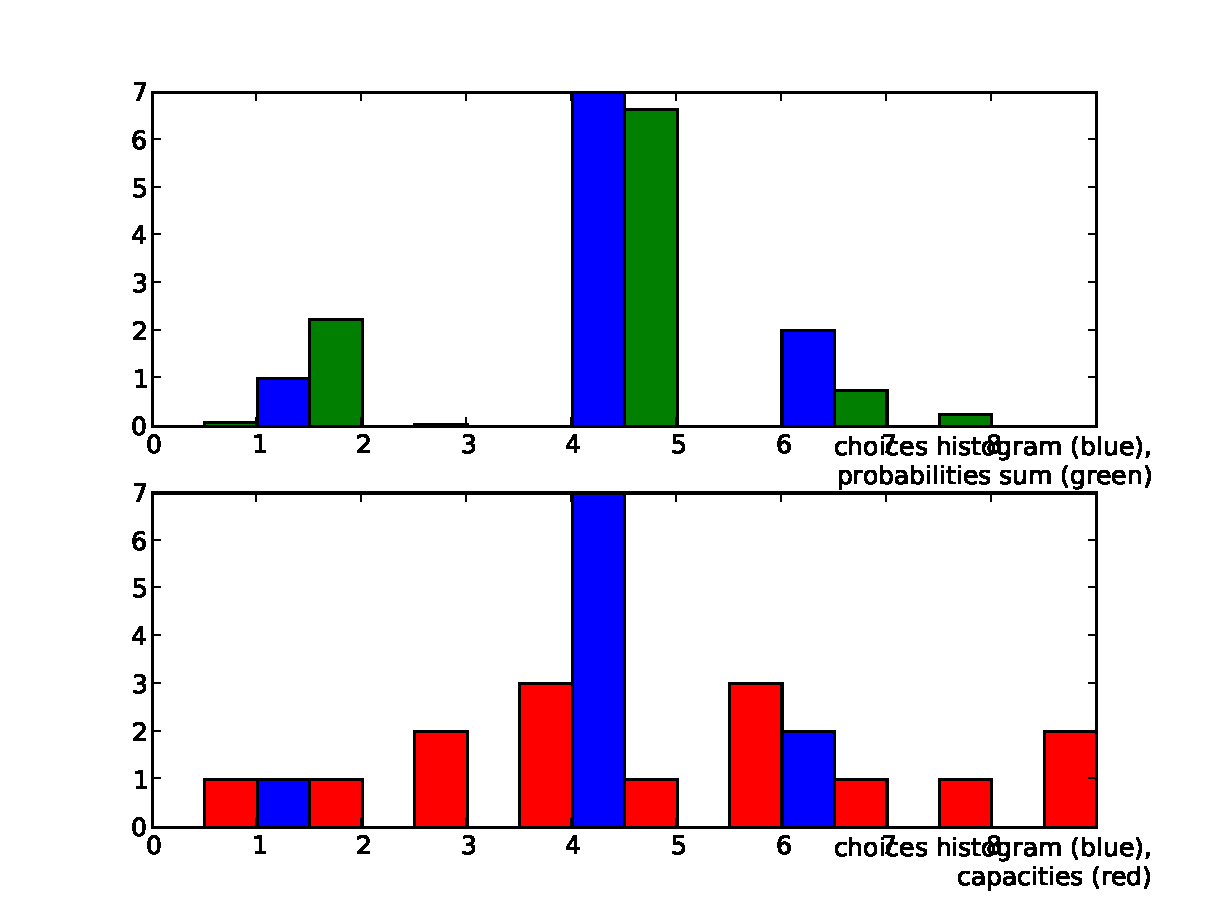
\includegraphics[scale=0.5, angle=0]{images/hlcmhist.pdf}
%end{latexonly}
\htmlonly{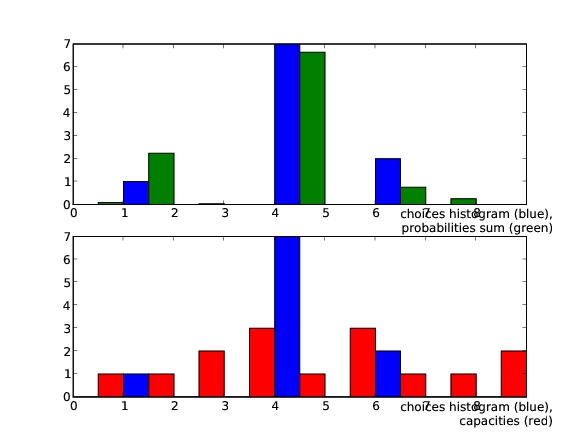
\includegraphics[scale=0.6, angle=0]{images/hlcmhist.jpg}}
\end{center}
In our case, more agents decided for the fifth and seventh location than there
are units available (which corresponds to the fact that those are two of the three cheapest locations).

In the above example, the discrete choice model consists of steps such as
computing utilities via the \class{opus_core.linear_utilities} class, computing
probabilities via the \class{opus_core.mnl_probabilities} class and computing
choices via the \class{opus_core.random_choices} class. These components
(default values) can be easily exchanged by other implementations. For
example, the class \class{urbansim.lottery_choices} for computing choices
takes into account capacity and forces agents to re-decide, if there is an
overflow in the locations capacity:
\begin{verbatim}
>>> number_of_agents = "gridcell.number_of_agents(household)"
>>> hlcm2 = HouseholdLocationChoiceModel(
                         location_set = locations,
                         sampler=None,
                         choices="urbansim.lottery_choices",
                         compute_capacity_flag=True,
                         capacity_string="capacity",
                         number_of_agents_string=number_of_agents,
                         number_of_units_string="capacity",
                         run_config={"lottery_max_iterations":10})
\end{verbatim}

The argument \verb|choices| is the full name of the module in which the choice
class is implemented. This module
must contain a class of the same name, i.e.
\class{lottery_choices} in this case, be a child of \package{opus_core} class \class{Choices}
(see Section~\ref{sec:choices}) and have a method \method{run()}.  Further arguments define the name of
the capacity attribute, \attributesindex name of the variable \variablesindex that computes number of agents in
each location (more about variable \variablesindex names in Section~\ref{sec:variable-names}), name of the
variable/attribute \attributesindex \variablesindex that determines the total number of units for each location. 
The argument \verb|run_config| is a dictionary that contains parameters for the simulation. In this example it contains a value
of how many times the households can re-decide if there is an overflow.

We run the above model:
\begin{verbatim}
>>> seed(1)
>>> result = hlcm2.run(specification, coefficients, households)
Running Household Location Choice Model 
                     (from urbansim.models.household_location_choice_model): 
                                            started on Wed Nov  5 18:18:58 2008
    Total number of individuals: 10
    HLCM chunk 1 out of 1.: started on Wed Nov  5 18:18:58 2008
        Number of agents in this chunk: 10
        Available capacity: 15.0 units.
        Number of unplaced agents: 0 (in 4 iterations)
    HLCM chunk 1 out of 1.: completed....................................0.0 sec
    gridcell.number_of_agents(household).................................0.0 sec
Running Household Location Choice Model 
     (from urbansim.models.household_location_choice_model): completed...0.0 sec
>>> hlcm2.plot_choice_histograms(capacity=locations.get_attribute("capacity"))
\end{verbatim}
\begin{center}
%begin{latexonly}
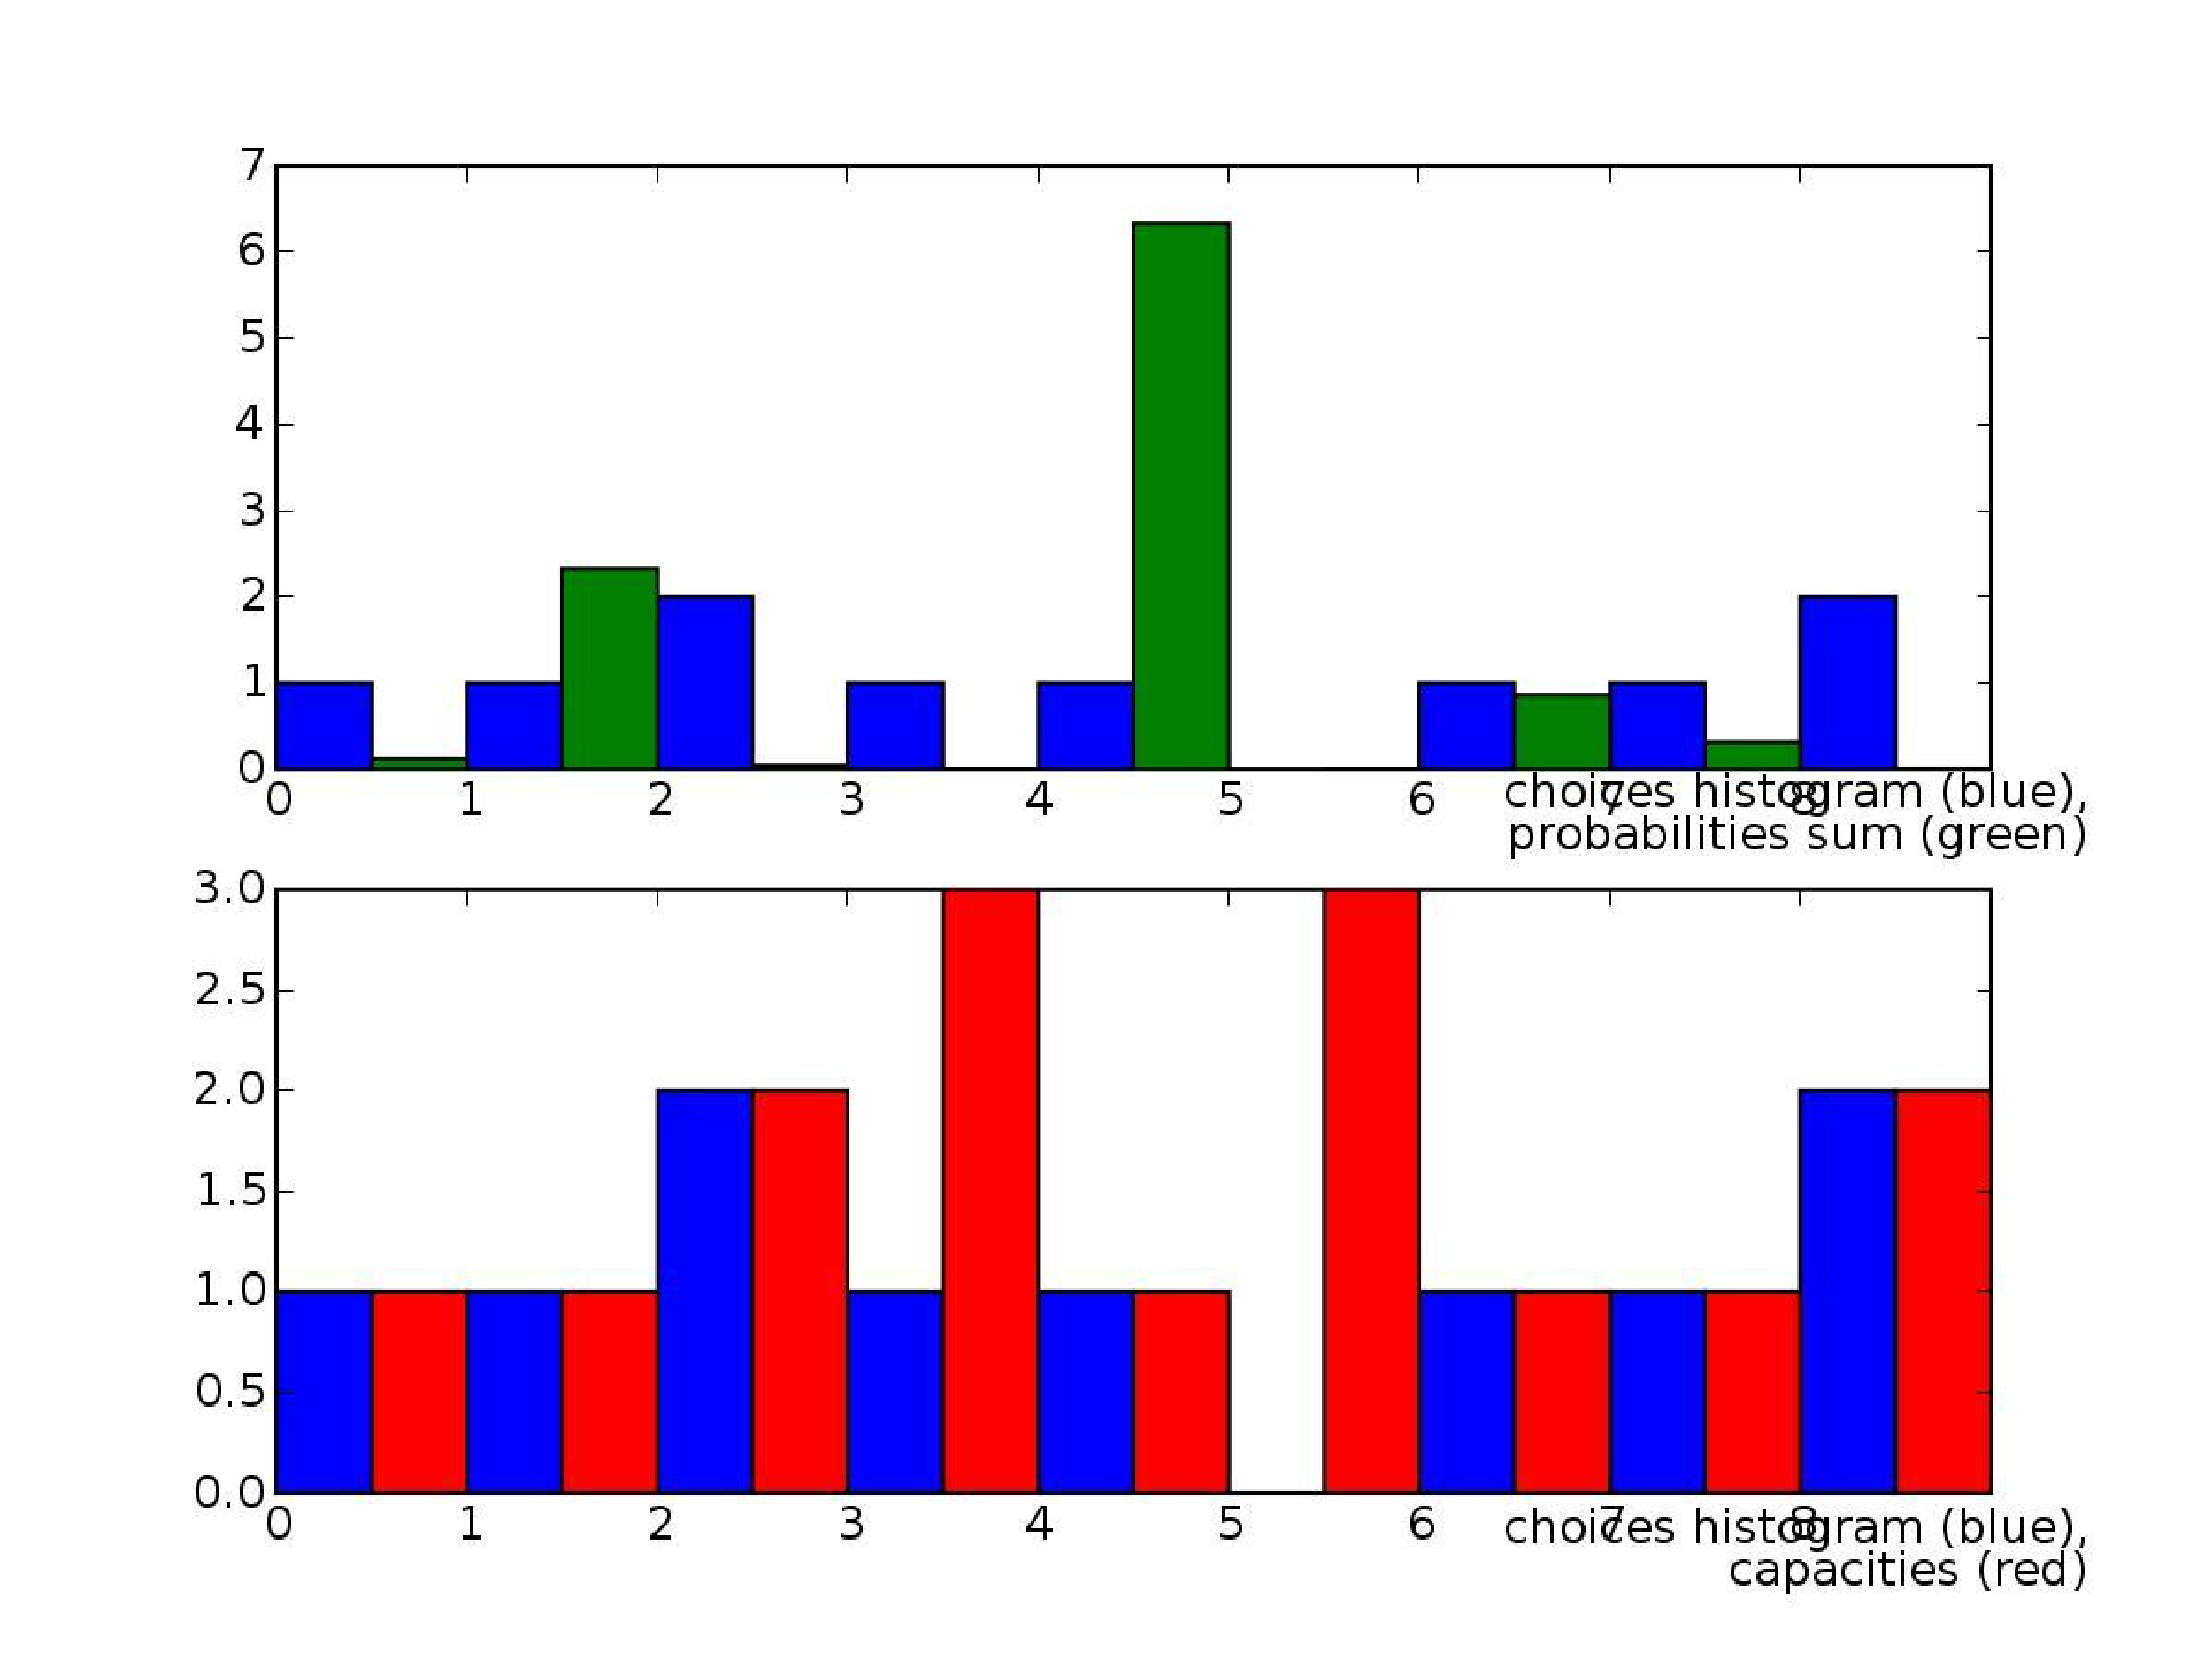
\includegraphics[scale=0.5, angle=0]{images/hlcm2hist.pdf}
%end{latexonly}
\htmlonly{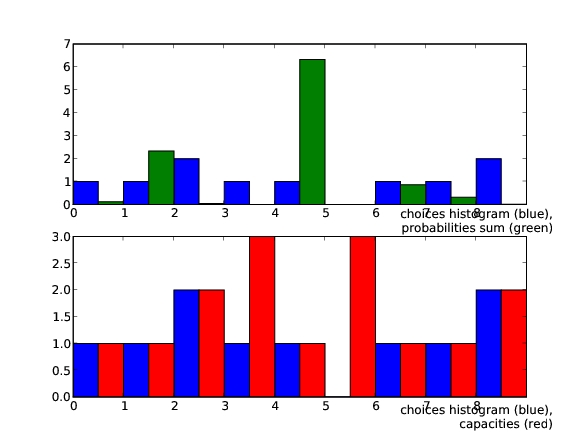
\includegraphics[scale=0.6, angle=0]{images/hlcm2hist.jpg}}
\end{center}
\attributesindex
\begin{verbatim}
>>> households.get_attribute("location")
array([9, 3, 9, 5, 4, 3, 7, 2, 8, 1])
\end{verbatim}
Now there is no overflow. Moreover, fourth and sixth locations still have free
units available, since they are the most expensive places. The agents were `forced'
to re-decide three times (i.e. 4 iterations in total). If the maximum
number of iterations given in \verb|run_config| would be reached without
placing all agents, the whole model would run automatically again. It would not be
very useful in this simple example, but the model is set-up for more complex situations,
including sampling of locations. Therefore in a new run, agents would sample
different locations which could solve the collision from the previous run.

Finally, agents that were not
placed have values smaller equal zero in the ``location'' attribute. \attributesindex

\package{urbansim} implements several location choice models.
Figure~\ref{fig:urbansim-model} in Section~\ref{sec:urbansim-models} shows
a hierarchical structure of the models.


%
\subsection{Regression Model}
%
\label{sec:RM}
%
Opus offers an infrastructure for estimation and simulation of a regression model
(see Section~\ref{sec:regression-model} for details).
Suppose our set of grid cells from the previous section has an attribute
``distance_to_cbd'' that contains information about the distance to the
central business district (cbd):

\begin{verbatim}
location cost  distance_to_cbd
1        500             5
2        200            10
3        600             5
4       1000             1
5        100            20
6       2000             0
7        300             7
8        400             7
9        800             3
\end{verbatim}

One can add the new attribute to the existing set of locations by:
\begin{verbatim}
>>> locations.add_primary_attribute(name="distance_to_cbd",
                                    data=[5,10,5,1,20,0,7,7,3])
\end{verbatim}

The cost of living in this dataset is highly correlated with
the distance to cbd and we can thus predict the cost using the regression model.

%
\subsubsection{Initialization}
%
The model is initialized by:
\begin{verbatim}
>>> from opus_core.regression_model import RegressionModel
>>> rm = RegressionModel(regression_procedure="opus_core.linear_regression")
\end{verbatim}
As in the case of choice model, the model is composed by model components, here
by plugging the appropriate regression procedure. The
regression procedure is a child of \class{Regression} (see Section~\ref{sec:regression}),
must have a method \method{run()} that gets as arguments a
multidimensional data array and a one-dimensional array of coefficients, \coefficientsindex and
returns a one-dimensional array of the regression outcome.

The \class{linear_regression} module implemented in \package{opus_core} is the default
procedure for the \class{RegressionModel} constructor and thus, it can be omitted.

%
\subsubsection{Estimation}
%
The specification for the above example consists of one variable \variablesindex and one
constant for the intercept:
\variablesindex
\begin{verbatim}
>>> specification = EquationSpecification(
                          variables=array(["constant", "gridcell.distance_to_cbd"]),
                          coefficients=array(["constant", "dcbd_coef"]))
\end{verbatim}
The estimation for predicting the cost of living is run by:
\begin{verbatim}
>> coef, other_results = rm.estimate(specification, dataset=locations,
                              outcome_attribute="gridcell.cost",
                              procedure="opus_core.estimate_linear_regression")
Estimating Regression Model (from opus_core.regression_model):
                                            started on Mon Mar 19 21:14:33 2007
    Estimate regression for submodel -2
    Number of observations: 9
    R-Squared:             0.536420010196
    Adjusted R-Squared:    0.470194297367
    Suggested |t-value| >  1.48230380737
    -----------------------------------------------
    Coeff_names estimate        SE      t-values
      constant   1114.07         213.758         5.21183
     dcbd_coef  -71.1493         24.9995        -2.84603
    ===============================================

Estimating Regression Model (from opus_core.regression_model): completed...0.4 sec
\end{verbatim}
The estimation procedure that is passed as an argument is expected to be
a child of \class{EstimationProcedure} (see Section~\ref{sec:estimation-procedure}) and have a
method \method{run()} that takes as arguments a
multidimensional data array and an instance of a class specified by the
argument \verb|regression_procedure| in the model constructor. Thus, the
estimation procedure can use the same code that is used for simulation.

The resulting object of class \class{Coefficients} \coefficientsindex called \verb|coef| can be stored or
directly used for predicting cost of other locations.
\coefficientsindex
\begin{verbatim}
>>> coef.summary()
Coefficient object:
size: 2
names: ['constant' 'dcbd_coef']
values:
[ 1114.07348633   -71.14933777]
standard errors:
[ 213.75848389   24.99952126]
t_statistic:
[ 5.211833   -2.84602809]
submodels: [-2 -2]
\end{verbatim}

%
\subsubsection{Simulation}
%
Suppose we have four locations with distance to cbd 2, 4, 6 and 8
respectively. We create a location dataset \datasetindex using
a storage type `dict'\index{Storage!dict}.
This type of storage is useful when we want to pass data directly without storing them on a physical storage media.

\begin{verbatim}
>>> dstorage = StorageFactory().get_storage('dict_storage')
>>> dstorage.write_table(table_name='gridcells',
                         table_data= {'id':array([1,2,3,4]),
                                      'distance_to_cbd':array([2,4,6,8])
                                    })
>>> ds = Dataset(in_storage=dstorage, in_table_name='gridcells',
                 id_name='id', dataset_name='gridcell')
\end{verbatim}
We have created a table in the RAM space called \file{gridcells} which is passed into the \class{Dataset} constructor.
Now we run the regression model with coefficients \coefficientsindex estimated in the previous
section:
\coefficientsindex \datasetindex
\begin{verbatim}
>>> cost = rm.run(specification, coefficients=coef, dataset=ds)
Running Regression Model (from opus_core.regression_model):
                                        started on Mon Mar 19 21:35:23 2007
    Total number of individuals: 4
    RM chunk 1 out of 1.: started on Mon Mar 19 21:35:23 2007
        Number of agents in this chunk: 4
    RM chunk 1 out of 1.: completed......................................0.0 sec
Running Regression Model (from opus_core.regression_model): completed....0.0 sec
>>> cost
array([ 971.77478027,  829.47613525,  687.17749023,  544.87878418])
\end{verbatim}
As expected, the resulting cost decreases with increasing distance to cbd.

%
\section{Opus Variables} \index{Variables!Opus}
%
\label{sec:variables}
%
\subsection{Variable Concept}
%
\label{sec:variableconcept}
%
\variablesindex

As mentioned in Section~\ref{sec:datasets}, a dataset \datasetindex has a set of
attributes, \attributesindex such as income or persons, that are stored in a file or database.
We call such characteristics \characteristicsindex {\it primary attributes}. \primaryattributesindex In addition, one is usually
interested in attributes \attributesindex that are computed, for example using some
transformation of primary attributes. \primaryattributesindex We call those attributes \attributesindex {\it
variables}, \variablesindex or {\it computed attributes}. \computedattributesindex They are simply handled as additional
``columns'' of a dataset \datasetindex to which they belong to, here denoted as
``parent dataset''. \datasetindex

In Opus, a variable \variablesindex is a class derived from the
\package{opus_core} class \class{Variable} \variablesindex.
(Section~\ref{sec:opus-variable} gives additional details about this class.)
Its name is identical to the name of the module in which it is implemented.
The module is stored in a directory whose name corresponds to the name of
the parent dataset. \datasetindex Note that the variable \variablesindex 
name must be all lower case.

The variable \variablesindex class must have a method \method{compute()} 
that returns a numpy array of
variable \variablesindex values. The size of that array must correspond to the number of entries in the parent
dataset. \datasetindex The \method{compute()} method takes an argument called
\verb|dataset_pool| containing references to the appropriate set of datasets to
use for computing this variable. From the \method{compute()} method, the parent dataset \datasetindex can be
accessed  by \method{self.get_dataset()}.

If the variable depends on other attributes, they must be listed in the method
\method{dependencies()}, which returns a list of all dependent variables and
attributes in their fully-qualified names (see
Section~\ref{sec:opus-core-attribute-names} for details on attribute
specification).

As an example, consider a variable ``is_in_wetland'' for the gridcell dataset
\verb|locations| from Sections~\ref{sec:LCM} and~\ref{sec:RM}. The variable
returns \verb|True| for entries whose percentage of wetland is more than a certain
threshold, and \verb|False| otherwise. The module \file{is_in_wetland.py},
containing a class \class{is_in_wetland}, is stored in the directory
\file{gridcell} because
\begin{verbatim}
>>> locations.get_dataset_name()
'gridcell'
\end{verbatim}

The class is defined as follows:
\variablesindex
\begin{verbatim}
from opus_core.variables.variable import Variable
class is_in_wetland(Variable):

    def dependencies(self):
        return ["gridcell.percent_wetland"]

    def compute(self, dataset_pool):
        return self.get_dataset().get_attribute("percent_wetland") > \
         dataset_pool.get_dataset('urbansim_constant')["percent_coverage_threshold"]

\end{verbatim}
The dependent attribute is a primary attribute and therefore specified as
a dataset-qualified name.  For our example, we populate the primary attribute:
\begin{verbatim}
>>> locations.add_primary_attribute(name="percent_wetland",
                                    data=[85,20,0,90,35,51,0,10,5])
\end{verbatim}

\subsubsection{Dataset Pool}
\index{dataset pool}
%
When computing variable values, Opus may need to access datasets used by
dependent variables, such as the \verb|urbansim_constant| dataset required by
\verb|is_in_wetland|, above.  These datasets are provided by the
\verb|dataset_pool| object passed into the variable's \method{compute} method.
This object is an instance of the \class{DatasetPool} class (see Section~\ref{sec:core-dataset-pool}).  It is responsible
for keeping a set of datasets for use when computing
variables.  If the requested dataset is in the pool already, it is returned
directly, otherwise it tries to find it in the given storage.

In order to find the appropriate dataset class for the requested dataset, the dataset
pool object searches the \file{datasets} directories of the Opus packages in
\verb|package_order|.  The first one to contain the appropriately named module
and class is used.  For instance, using the \verb|storage| object created on page~\pageref{storagepage},
for the definition:
\begin{verbatim}
>>> from opus_core.dataset_pool import DatasetPool
>>> dataset_pool = DatasetPool(package_order=['urbansim', 'opus_core'],
                               storage=storage)
\end{verbatim}
if \verb|dataset_pool| is asked for the ``household'' dataset, and does not
already have one in its pool, it will look in the \verb|storage|. In order to
create the corresponding dataset classes
it searches for a file
\file{household_dataset.py} (containing the class \class{HouseholdDataset}) first in \file{urbansim/datasets} and then in
\file{opus_core/datasets}. The first one found will be used.
\begin{verbatim}
>>> dataset_pool.datasets_in_pool()
{}
>>> hs = dataset_pool.get_dataset("household")
>>> dataset_pool.datasets_in_pool()
{'household': <urbansim.datasets.household_dataset.HouseholdDataset object
                                                               at 0x197c2f70>}
>>> hs.size()
10
\end{verbatim}
If the dataset pool is asked for \verb|urbansim_constant| and `urbansim' is included in \verb|package_order|,
it will use some \package{urbansim} specific constants defined in \file{urbansim/constants.py} (in addition to
user defined constants found on storage).

For the purpose of this example, we set the required constant by:
\begin{verbatim}
>>> constant = dataset_pool.get_dataset("urbansim_constant")
>>> constant["percent_coverage_threshold"] = 50
\end{verbatim}

\subsubsection{Invoking Computation}
\label{sec:compute-variables}
Computation of a variable is invoked using the \class{Dataset} method
\method{compute_variables()} passing the variable name in its fully-qualified
form and a dataset pool if other datasets are required for this variable:
 \label{page:compute-isnearcbd}
\variablesindex
\begin{verbatim}
>>> locations.compute_variables("urbansim.gridcell.is_in_wetland",
                                  dataset_pool=dataset_pool)
urbansim.gridcell.is_in_wetland..........................................0.0 sec
array([ True, False, False,  True, False,  True, False, False, False], dtype=bool)
\end{verbatim}

The method returns the resulting values of the variable. The
\verb|compute_variables| method also accepts a list of variables to be
computed.  In this case it returns values of the last variable in the list.

 In addition, within the dataset, the variable can be accessed using its un-qualified name.
 Thus, the un-qualified names of variables including the primary
 attributes must be unique.
\begin{verbatim}
>>> locations.get_attribute("is_in_wetland")
array([ True, False, False,  True, False,  True, False, False, False], dtype=bool)
\end{verbatim}

\subsection{Interaction Variables}
\label{sec:interactions}

In order to work with variables \variablesindex that determine an
interaction between two datasets, \datasetindex there is a subclass of
\class{Dataset}, called
\class{InteractionDataset}. Attributes of this class are stored as
two-dimensional arrays (see Section~\ref{sec:interaction-set} for details).

To create an interaction set for households and gridcells from the previous
sections, do
\begin{verbatim}
>>> from opus_core.datasets.interaction_dataset import InteractionDataset
>>> interactions = InteractionDataset(dataset1 = households, dataset2 = locations)
\end{verbatim}
The dataset name is composed from dataset names of the two interacting datasets: \datasetindex
\begin{verbatim}
>>> interactions.get_dataset_name()
'household_x_gridcell'
\end{verbatim}
Thus, an interaction variable \variablesindex for such dataset \datasetindex will be implemented in the
directory \file{household_x_gridcell}.

The \class{InteractionDataset} class contains several methods that are useful for
variable \variablesindex computation which must return a two-dimensional array. For example, a
variable \variablesindex defined as a multiplication of cost and income can be implemented as:
\variablesindex
\begin{verbatim}
from opus_core.variables.variable import Variable

class cost_times_income(Variable):
    def dependencies(self):
        return ["gridcell.cost", "household.income"]

    def compute(self, dataset_pool):
        return self.get_dataset().multiply("income", "cost")
\end{verbatim}

This \class{cost_times_income} variable is mostly for illustration; it can
also be defined more conveniently as an expression (see Section
\ref{sec:urbansim-tutorial-expressions}).

If we wish that only a subset of each dataset \datasetindex interact (for example for
memory reasons), we can pass the corresponding indices to the constructor:
\index{Memory!Loading a subset of a dataset}
\begin{verbatim}
>>> from numpy import arange
>>> interactions = InteractionDataset(dataset1 = households, dataset2 = locations,
                                  index1 = arange(5), index2 = arange(3))
\end{verbatim}
Here only the first 5 households and the first three gridcells interact.
The \method{compute()} method of the interaction variable \variablesindex should return an array of
size index1 $\times$ index2.

\variablesindex \attributesindex
\begin{verbatim}
>>> interactions.compute_variables(
        ["urbansim.household_x_gridcell.cost_times_income"])
array([[  500000.,   200000.,   600000.],
       [ 1000000.,   400000.,  1200000.],
       [ 2500000.,  1000000.,  3000000.],
       [ 1500000.,   600000.,  1800000.],
       [  250000.,   100000.,   300000.]])
\end{verbatim}
\label{page:compute-interaction}

\package{urbansim} uses interaction variables \variablesindex mainly in \class{ChoiceModel} classes, where agents
interact with dataset \datasetindex of choices. The household location choice model object
\verb|hlcm| from Section~\ref{sec:LCM} can be for example estimated using two
variables, \variablesindex one of which is an interaction variable: \variablesindex
\primaryattributesindex
\begin{verbatim}
>>> specification = EquationSpecification(
                     variables=array([
                          "gridcell.cost",
                          "urbansim.household_x_gridcell.cost_times_income"]),
                     coefficients=array(["costcoef", "cti_coef"]))
>>> # place households
>>> households.add_primary_attribute(data=[2,8,3,1,5,4,9,7,3,6], name="location")
>>> coef, other_results = hlcm.estimate(specification, households)
Estimating Household Location Choice Model 
                     (from urbansim.models.household_location_choice_model): 
                                             started on Thu Nov  6 12:12:47 2008
    urbansim.household_x_gridcell.cost_times_income......................0.0 sec
    submodel: -2
    Convergence achieved.
    Akaike's Information Criterion (AIC):  39.8199022026
    Number of Iterations:  18
    ***********************************************
    Log-likelihood is:            -17.9099511013
    Null Log-likelihood is:       -21.9722457734
    Likelihood ratio index:       0.184882998032
    Adj. likelihood ratio index:  0.0938590753688
    Number of observations:       10
    Suggested |t-value| >         1.51742712939
    Convergence statistic is:     0.000302603242051
    -----------------------------------------------
    Coeff_names estimate        std err         t-values
      costcoef  -0.00312452     0.00339464      -0.920429
      cti_coef  4.45803e-07     5.34429e-07     0.834168
    ***********************************************
    Elapsed time:  0.02 seconds
Estimating Household Location Choice Model 
     (from urbansim.models.household_location_choice_model): completed...0.0 sec
\end{verbatim}
\coefficientsindex
\label{page:iv-spec}

%
\subsection{Versioning}
\label{sec:versioning}
%
Opus uses a mechanism of versioning of variables \variablesindex and attributes. \attributesindex Each
variable/attribute \variablesindex\attributesindex is initialized with a version number 0. Any subsequent
change of that variable/attribute \variablesindex\attributesindex increments the version number. This allow us
to only recompute variables, \variablesindex if it is really needed. This means that if a
computation is invoked (by e.g.\ \verb|compute_variables()|), \variablesindex it is checked, if
any of the version numbers of all dependent variables \variablesindex has changed since the
last computation. The computation is performed only, if there was any change
in the dependencies tree. The mechanism is described in Section~\ref{sec:dependencies-tree}
in more detail.

For example,
\variablesindex
\begin{verbatim}
>>> households.get_version("income")
0
>>> res = interactions.compute_variables([
             "urbansim.household_x_gridcell.cost_times_income"])
>>> interactions.get_version("cost_times_income")
0
>>> households.modify_attribute(name="income", data=[14000], index=[9])
>>> households.get_version("income")
1
>>> res = interactions.compute_variables([
             "urbansim.household_x_gridcell.cost_times_income"])
urbansim.household_x_gridcell.cost_times_income.......................0.0 sec
>>> interactions.get_version("cost_times_income")
1
\end{verbatim}

The first call of \method{compute_variables()} didn't perform the actual
computation, because nothing has changed since our previous computation on
page~\pageref{page:compute-interaction}.
After we modify one element of the ``income'' attribute
(note that ``income'' is a dependent variable of
``cost_times_income'' defined in the \method{dependencies()} method), the
variable is recomputed and the version number is increased.

\subsection{Using Arguments in Variable Names}
\label{sec:tutorial-numbersinvariables}

Opus offers the possibility of including a number or a character string into
variable name which is then passed to the variable constructor as an argument.
The module/class name of such variable corresponds to a pattern in which a
number is replaced by `DDD' and a string is replaced by `SSS'\@.  For example,
a similar variable to \class{is_in_wetland} in Section~\ref{sec:variableconcept} can be
implemented in a way that the threshold is directly included in the variable
name, such as \\
\class{is_in_wetland_if_threshold_is_80}. Here, we give an example of variable
of the type \verb|is_near_|{\em location}\verb|_if_threshold_is_|{\em number}.
As {\em location} we can use e.g. `highway',  `arterial', or `cbd'.
The class name is \class{is_near_SSS_if_threshold_is_DDD} and must have a
constructor implemented which takes a string and a number as arguments:

\variablesindex
\numpyindex
\begin{verbatim}
from opus_core.variables.variable import Variable

class is_near_SSS_if_threshold_is_DDD(Variable):
    def __init__(self, location, number):
        self.location = location
        self.number = number
        Variable.__init__(self)

    def dependencies(self):
        return ["gridcell.distance_to_" + self.location]

    def compute(self, dataset_pool):
        distance_to_location = self.get_dataset().get_attribute(
                                        "distance_to_" + self.location)
        return distance_to_location < self.number
\end{verbatim}
We can then invoke the computation for the `cbd' location and different
thresholds by changing the variable name:
\begin{verbatim}
>>> res = locations.compute_variables(
      map(lambda threshold:
       "urbansim.gridcell.is_near_cbd_if_threshold_is_%s" % threshold, [2,4,7]))
urbansim.gridcell.is_near_SSS_if_threshold_is_DDD...................0.0 sec
urbansim.gridcell.is_near_SSS_if_threshold_is_DDD...................0.0 sec
urbansim.gridcell.is_near_SSS_if_threshold_is_DDD...................0.0 sec
\end{verbatim}

\attributesindex
\begin{verbatim}
>>> locations.get_attribute("is_near_cbd_if_threshold_is_2")
array([False, False, False,  True, False,  True, False, False, False], dtype=bool)
>>> locations.get_attribute("is_near_cbd_if_threshold_is_4")
array([False, False, False,  True, False,  True, False, False,  True], dtype=bool)
>>> locations.get_attribute("is_near_cbd_if_threshold_is_7")
array([ True, False,  True,  True, False,  True, False, False,  True], dtype=bool)
\end{verbatim}

If the dataset \datasetindex \verb|locations| would have an attribute \attributesindex
``distance_to_highway'', we
could use the same variable \variablesindex implementation for variables \variablesindex
\class{is_near_highway_if_threshold_is_...}.

The arguments of the constructor are passed in the same number and order as
they appear in the variable name. For example, if the name would contain only
one pattern, say DDD, the constructor would expect only one argument, namely
an integer. The method \method{dependencies()} is called from
\method{Variable.__init__()}, therefore any class attributes used in
\method{dependencies()} (such as \verb|self.location| in this case) must be set
before the call of \\
\method{Variable.__init__()}.

\emph{Note: Arguments for variable names will probably be replaced with a
  more standard syntax in the future, for example
  \class{is_near(feature='highway', threshhold=2)}.  However, we don't have
  a specific date yet for this change.  We will try to preserve backward
  compatibility.}

\section{Expressions}
\label{sec:urbansim-tutorial-expressions}
\index{expressions}

In many cases variable definitions are simple expressions involving other
variables.  For these cases, Opus provides an \emph{expression language}
that allows them to be defined succinctly, rather than requiring the Opus
user to write new variable definitions in Python.  (The expression language
has been added recently to Opus, and there are many explicitly declared
variables in the existing UrbanSim package that are no longer needed ---
they could be written as expressions instead in the specifications.  We
plan to remove these unneeded variables in the future.)

The syntax of the expression language is that of Python, but the semantics
are somewhat different --- for example, a name like
\code{gridcell.distance_to_cbd} is a reference to the value of that
variable.  (If you just evaluated this in a Python shell you'd get an
error, saying that the \package{gridcell} package didn't have a
\code{distance_to_cbd} attribute.)  Here is a simple example:

\begin{verbatim}
>>> locations.compute_variables(["sqrt(gridcell.distance_to_cbd)"])
array([ 2.23606798,  3.16227766,  2.23606798,  1.        ,  4.47213595,
        0.        ,  2.64575131,  2.64575131,  1.73205081])
\end{verbatim}

The expressions are fed to the \method{compute_variables} method 
\index{compute_variables} of
\class{Dataset} (Section \ref{sec:compute-variables}), just as for simple
variable references.  (In fact, given a new expression, Opus will compose a
new variable definition, including a \method{compute} and a
\method{dependencies} method, which computes the value of that expression.
It then saves the new variable definition in case the same expression is
encountered again.  However, the user need not
be concerned about this.)  The \method{compute_variables} method evaluates
each variable (or expression) in turn, and returns the value of the last one.

An expression consists of an attribute name, or a function or operation
applied to other expressions.  This definition is recursive, so that a
function or operation can be applied to expressions composed
from other expressions.  For example, here are some legal expressions:

\begin{itemize}

\item \code{urbansim.gridcell.population}
\item \code{ln(urbansim.gridcell.population)+1}

\end{itemize}

\subsection{Variable Names in Expressions}

The name used in an expression can be either a fully-qualified variable
name, a dataset-qualified variable name, or a primary attribute.
The variable names can include arguments (Section
\ref{sec:tutorial-numbersinvariables}), \index{arguments}
so that
\class{is_near_highway_if_threshold_is_2} matches the variable definition
for \class{is_near_SSS_if_threshold_is_DDD}.

\subsection{Unary Functions for Opus Expressions}
\label{sec:functions-for-opus-expressions}

There is a set of unary functions defined to use in expressions, as
follows.  These all operate on numpy arrays.

\begin{description}

\item[\code{clip_to_zero}] Returns the input values with all negative values
   clipped to 0. \index{clip_to_zero}

\item[\code{exp}] Returns an array consisting of $e$ raised to the input 
values.\index{exp}

\item[\code{ln}] Returns an array of natural logarithms.  Input values of 0
result in 0.  (The intent is that this function be used on arrays of
values, where 0 denotes a missing value.  However, be cautious --- as you
approach 0 from the positive side, the result value becomes more and more
negative, and then suddenly returns to 0 at 0.)  \index{ln}

\item[\code{ln_bounded}] Returns an array of natural logarithms. Values
less than 1 result in 0.  \index{ln_bounded}

\item[\code{ln_shifted}] Returns an array of natural logarithms.  The input
  values are shifted by the second argument before taking the log.  (The
  default shift value is 1.)  \index{ln_shifted}

\item[\code{ln_shifted_auto}] If the input values includes values that are
less than or equal to 0, they are shifted so that the minimum of the
shifted values is 1 before taking the log.  Otherwise the log is taken on
the original values.  \index{ln_shifted_auto}

\item[\code{sqrt}] Returns an array of square roots.  Values less than 0
  result in 0. \index{sqrt}

\item[\code{safe_array_divide}] First three arguments are the nominator, denominator and 
a constant. The function returns an array of numerator / denominator for all values where denominator is not 0,
otherwise the constant (default value is 0). An optional fourth argument controls
the type of the resulting array. The default value is 'float32'.
\end{description}

In addition, all of the functions in numpy are available.  To avoid name
collisions, the function name in an expression must include the package
name \code{numpy}.  For example, this expression gives you the reciprocals
of all the values in a variable \code{v}:

\code{numpy.reciprocal(v)}

\subsection{Operators for Opus Expressions}
\index{numpy!operators}

All of the numpy operators can be used in Opus expressions, including
\verb|+ - * / ** |.  Note the numpy semantics for these --- for example,
\verb|*| does elementwise multiplication of two numpy arrays, or with a
scalar argument, scales all the elements in an array,
e.g.\ \code{1.2*household.income}.

\subsection{Aliasing}
\label{sec:aliasing}
\index{aliasing}

A new attribute name can be declared and initialized using an assignment
statement:

\code{lnpop = ln(urbansim.gridcell.population)}

This is treated as an expression, which can occur in the list of
expressions given to \method{compute_variables} or in an \file{aliases.py}
file (see below).  The value of the new alias is returned as the value of
the expression if it's the last item on the list of variables and
expressions.

It is convenient, and often more efficient, to gather all the expressions
and aliases for a particular package and dataset into one place.  The
optional \file{aliases.py} file supports this.  \index{alias.py file}
This file should define a
single variable \code{aliases} to be a list of expressions, each of which
should define an alias.  This file is then placed in the same directory as
variables for that package and dataset.  For example, to define aliases
relevant to \code{urbansim.gridcell}, put an \file{aliases.py} file into
the \file{urbansim.gridcell} directory.  These aliases can then be referred
to using the fully-qualified name of the alias.  When finding a variable
referenced by a fully-qualified name, the system first searches the aliases
file (if present), and then the variable definitions in the appropriate
directory.

As an example, the directory \code{opus_core.test_agent} contains one
variable definition, for the variable \code{income_times_2}.  (This
directory and variable are used for unit tests for \package{opus_core}.)
The file \file{aliases.py} in that same directory contains the following:

\begin{verbatim}
aliases = [
    'income_times_5 = 5*opus_core.test_agent.income',
    'income_times_10 = 5*opus_core.test_agent.income_times_2'
    ]
\end{verbatim}

The first alias refers to a primary attribute (\code{test_agent.income}),
and the second to the variable.  These aliases can then be referred to
using a fully-qualified name, in exactly the same way as a variable,
for example

\code{opus_core.test_agent.income_times_5}.  

See the unit tests in
\file{opus_core.variables.expression_tests.aliases_file} for examples of
using these aliases.

\subsection{Casting the Value of an Expression}
\index{casting}

Normally the value of a variable defined by an expressions will be a
\code{float64} (this is a numpy type).  For large datasets this may use too
much space.  You can cast the result of any expression to a different type
using the numpy \code{astype} method.  For example, the alias defined by
this expression will be of type \code{float32}:

\begin{verbatim}
lnpop = ( ln(urbansim.gridcell.population) ).astype(float32)
\end{verbatim}

The following numpy types can be used as the argument to the \code{astype}
method: \code{bool8}, \code{int8}, \code{uint8}, \code{int16},
\code{uint16}, \code{int32}, \code{uint32}, \code{int64}, \code{uint64}
\code{float32}, \code{float64}, \code{complex64}, \code{complex128}, and
\code{longlong}.
 
\subsection{Interaction Sets}
\index{interaction sets}

If you access an attribute of a component of an interaction set in the
context of that interaction set, the result is converted into a 2-d array
and returned.  These 2-d arrays can then be multiplied, divided, compared,
and so forth, using the numpy functions and operators.  For example,
suppose we have an interaction set \file{household_x_gridcell}.  The
component \file{household} set has an attribute \verb|income| with values
\verb|[100, 200, 300]|.  (These numbers are just to explain the concepts
--- obviously they aren't realistic incomes.)  The \file{gridcell}
component has an attribute \verb|cost| with values \verb|[1000, 1200]|.
Then evaluating

\begin{verbatim}
household_x_gridcell.compute_variables('urbansim.household.income')
\end{verbatim}

will return a 2-d array

\begin{verbatim}
[ [100, 100],
  [200, 200],
  [300, 300] ]
\end{verbatim}

and

\begin{verbatim}
household_x_gridcell.compute_variables('urbansim.gridcell.cost')
\end{verbatim}

returns

\begin{verbatim}
[ [1000, 1200],
  [1000, 1200],
  [1000, 1200] ]
\end{verbatim}

Then
\begin{verbatim}
household_x_gridcell.compute_variables(
            'urbansim.gridcell.cost*urbansim.household.income')
\end{verbatim}

evaluates to
\begin{verbatim}
[ [100000, 120000],
  [200000, 240000],
  [300000, 360000] ]
\end{verbatim}

Both the arguments to the operation and the result can be used in more
complex expressions.  For example, if we wanted to give everyone
a \$5000 income boost, and also scale the result, this could be done using
\verb|(household.income+5000)*gridcell.cost * 1.2|.

As another example, the model specification from
page~\pageref{page:iv-spec} can be modified by using an expression for the
interaction and taking its log: \variablesindex \coefficientsindex

\begin{verbatim}
>>> specification = EquationSpecification(
      variables=("gridcell.cost",
         "ln(urbansim.gridcell.cost*urbansim.household.income)"),
      coefficients=("costcoef", "cti_coef"))
\end{verbatim}


\subsection{Aggregation and Disaggregation}
\label{sec:aggregation}
\index{aggregation} \index{disaggregation}

The methods \class{aggregate} and \class{disaggregate} are used to
aggregate and disaggregate variable values over two or more datasets.  
\index{aggregate} \index{disaggregate} The \class{aggregate} method associates
information from one dataset to another along a many-to-one relationship, while
the \class{disaggregate} method does the same along a one-to-many relationship. Some
examples are:

\begin{itemize}
\item \code{zone.aggregate(gridcell.population)}

\item \code{zone.aggregate(2.5*gridcell.population)}

\item \code{zone.aggregate(urbansim.gridcell.population)}

\item \code{neighborhood.aggregate(gridcell.population, 
  intermediates=[zone,faz])}

\item \code{neighborhood.aggregate(gridcell.population, 
  intermediates=[zone, faz], function=mean)}

\item \code{zone.aggregate(gridcell.population, function=mean)}

\item \code{region.aggregate_all(zone.my_variable)}

\item \code{region.aggregate_all(zone.my_variable, function=mean)}

\item \code{faz.disaggregate(neighborhood.population)}

\item \code{gridcell.disaggregate(neighborhood.population, 
      intermediates=[zone, faz])}

\end{itemize}

The syntax and semantics for these is as follows.

\subsubsection{Aggregation}

Suppose we have three different geographical units: gridcells, zones and
neighborhoods.  We have information available on the gridcell level and
would like to aggregate this information for zones and neighborhoods. We
know the assignments of gridcells to zones and of zones to neighborhoods.

First, we place the data for three neighborhoods and five zones into a dict storage:\index{Storage!dict}
\begin{verbatim}
>>> dstorage = StorageFactory().get_storage('dict_storage')
>>> dstorage.write_table(table_name='neighborhoods',
                         table_data={"nbh_id":array([1,2,3])}
                         )
>>> dstorage.write_table(table_name='zones',
                         table_data={"zone_id":array([1,2,3,4,5]),
                                     "nbh_id": array([3,3,1,2,1])}
                         )
\end{verbatim}

Then, we create the corresponding datasets: \datasetindex
\begin{verbatim}
>>> neighborhoods = Dataset(in_storage=dstorage, in_table_name='neighborhoods',
                            dataset_name="neighborhood", id_name="nbh_id")
>>> zones = Dataset(in_storage=dstorage, in_table_name='zones',
                    dataset_name="zone", id_name="zone_id")
\end{verbatim}
Note that \verb|zones| contain assignments to neighborhoods in the
attribute `nbh_id'.  For the gridcell set, consider the dataset \datasetindex
\verb|locations| defined on page~\pageref{page:tutorial-gc-locations}. We
add assignments of those nine locations to the zones:
\primaryattributesindex
\begin{verbatim}
>>> locations.add_primary_attribute(name="zone_id", data=[3,5,2,2,1,1,3,5,3])
\end{verbatim}
Note that any assignment must be done by using an attribute \attributesindex of the same name
as the unique identifier of the dataset \datasetindex that the assignment is made to.

As the next step, we prepare a dataset pool \index{dataset pool} for the variable computation, since we are dealing with variables
that involve more than one dataset. To make things easy, we explicitly insert
our three datasets into the pool:
\begin{verbatim}
>>> dataset_pool = DatasetPool(package_order=['urbansim', 'opus_core'],
                               datasets_dict={'gridcell': locations,
                                              'zone': zones, 
                                              'neighborhood':neighborhoods})
\end{verbatim}
An aggregation over one geographical level for the \verb|locations|
attribute \attributesindex `capacity' can be done by: \variablesindex
\attributesindex
\begin{verbatim}
>>> aggr_var = "aggregated_capacity = zone.aggregate(gridcell.capacity)"
>>> zones.compute_variables(aggr_var, dataset_pool=dataset_pool)
aggregated_capacity = zone.aggregate(gridcell.capacity)..................0.0 sec
array([ 4.,  5.,  4.,  0.,  2.])
\end{verbatim}
By default, the aggregation function applied to the aggregated data is the
`sum' function. This can be changed by passing the desired function as second
argument in the variable \variablesindex name: \variablesindex
\begin{verbatim}
>>> aggr_var = \
"zone.aggregate(urbansim.gridcell.is_near_cbd_if_threshold_is_2, function=maximum)"
>>> zones.compute_variables(aggr_var, dataset_pool=dataset_pool)
zone.aggregate(urbansim.gridcell.is_near_cbd_if_threshold_is_2, function=maximum):
                                                            completed...0.4 sec
array([ 1.,  1.,  0.,  0.,  0.])
\end{verbatim}

The \method{aggregate} method accepts the following aggregation functions:
sum, mean, variance, standard_deviation, minimum, maximum,
center_of_mass. These are functions of the scipy package
\module{ndimage}.

An aggregation over two or more levels of geography is done by passing a
third argument into the \class{aggregate} method. It is a list of dataset
\datasetindex names over which it is aggregated, excluding datasets
\datasetindex for the lowest and highest level. For example, aggregating
the gridcell attribute \attributesindex `capacity' for the neighborhood set
can be done by: \variablesindex \attributesindex
\begin{verbatim}
>>> aggr_var2 = \
   "neighborhood.aggregate(gridcell.capacity, function=sum, intermediates=[zone])"
>>> neighborhoods.compute_variables(aggr_var2, dataset_pool=dataset_pool)
neighborhood.aggregate(gridcell.capacity, function=sum, intermediates=[zone])
    zone.aggregate(gridcell.capacity,function=sum).......................0.0 sec
neighborhood.aggregate(gridcell.capacity, function=sum, intermediates=[zone]):
                                                            completed...0.3 sec
array([ 6.,  0.,  9.])
\end{verbatim}

\subsubsection{Disaggregation}

Disaggregation is done analogously. The \class{disaggregate} method takes
information from a coarse set of entities and allocates it to a finer set of
entities, in the manner of a one-to-many relationship. By default, the function
for allocating data is to simply replicate the data on the parent entity for
each inheriting entity. The method takes one required argument, an
attribute/variable
\attributesindex\variablesindex name, and one optional argument, a list of
dataset \datasetindex names. Here we add an attribute \attributesindex
``is_cbd'' to the neighborhood set and distribute it across gridcells:
\primaryattributesindex \variablesindex
\begin{verbatim}
>>> neighborhoods.add_primary_attribute(name="is_cbd", data=[0,0,1])
>>> disaggr_var = \
       "is_cbd = gridcell.disaggregate(neighborhood.is_cbd, intermediates=[zone])"
>>> locations.compute_variables(disaggr_var, dataset_pool=dataset_pool)
is_cbd = gridcell.disaggregate(neighborhood.is_cbd, intermediates=[zone])
    zone.disaggregate(neighborhood.is_cbd).......................0.0 sec
is_cbd = gridcell.disaggregate(neighborhood.is_cbd, intermediates=[zone]):
                                                           completed...0.0 sec
array([0, 0, 1, 1, 1, 1, 0, 0, 0])

\end{verbatim}

Note that since we used the dataset-qualified \datasetindex name for
``is_cbd'' in the \method{disaggregate} method, the attribute must be a
primary attribute \primaryattributesindex of \verb|neighborhoods|.  The
\method{aggregate} and \method{disaggregate} methods both must have the
dataset name of the dataset for which they are computed before the method
name, e.g.\ \code{gridcell.disaggregate}.

To aggregate over all members of one dataset, \datasetindex one can use the
built-in method \method{aggregate_all}. It must be used with a dataset
\datasetindex that has one element which is the case of the
\package{opus_core} dataset \datasetindex \class{AlldataDataset}
implemented in the directory \file{datasets}. For example, the total
capacity for all gridcells can be determined by: \variablesindex
\attributesindex
\begin{verbatim}
>>> from opus_core.datasets.alldata_dataset import AlldataDataset
>>> alldata = AlldataDataset()
>>> alldata.compute_variables(
        "total_capacity = alldata.aggregate_all(gridcell.capacity, function=sum)",
        dataset_pool=dataset_pool)
total_capacity = alldata.aggregate_all(gridcell.capacity, function=sum)....0.0 sec
array([ 15.])
\end{verbatim}
In addition to \method{sum}, the \class{aggregate_all} class accepts all
functions that are accepted by the \class{aggregate} class;
the default is \method{sum}.

If the attribute being aggregated or disaggregated is a simple variable, it
should be either dataset-qualified or fully-qualified, i.e.\ always
including the dataset name and optionally including the package name.  The
attribute being aggregated can also be an expression.  (In this case,
behind the scenes the system generates a new variable for that expression,
and then uses the new variable in the aggregation or disaggregation
operations.  However, this isn't visible to the user.)  The result of an
aggregation or disaggregation can also be used in more complex expressions,
e.g. \code{ln(2*aggregate(gridcell.population))}.

\subsection{Number of Agents}
\index{number_of_agents}

A common task in modeling is to determine a number of agents of one dataset
\datasetindex that are assigned to another dataset. \datasetindex For this
purpose, Opus contains a built-in method \class{number_of_agents}, which
takes as an argument the name of the agent dataset. \datasetindex For
example, our household dataset \datasetindex is assigned to the following
locations: \attributesindex
\begin{verbatim}
>>> households.modify_attribute(name="location",
                              data=[2, 8, 3, 1, 5, 4, 9, 7, 3, 6])
\end{verbatim}
Then, the number of households in each location can be determined by:
\variablesindex \attributesindex
\begin{verbatim}
>>> dataset_pool.add_datasets_if_not_included({'household': households})
>>> locations.compute_variables("gridcell.number_of_agents(household)",
                                dataset_pool=dataset_pool)
gridcell.number_of_agents(household).....................0.0 sec
array([ 1.,  1.,  2.,  1.,  1.,  1.,  1.,  1.,  1.])
\end{verbatim}
Note that we had to add the household dataset to the dataset pool \index{dataset pool}
in order to have it available in the computation process.

Similarly, the number of zones in neighborhoods is computed by
\variablesindex\attributesindex
\begin{verbatim}
>>> neighborhoods.compute_variables("neighborhood.number_of_agents(zone)",
                                    dataset_pool=dataset_pool)
neighborhood.number_of_agents(zone)......................0.0 sec
array([ 2.,  1.,  2.])
\end{verbatim}

As in the case of \method{aggregate} and \method{disaggregate}, the
\method{number_of_agents} method must be preceded by the `owner' dataset
name, e.g. \verb|neighborhood.number_of_agents| for computing on the
\verb|neighborhood| dataset.

%
\section{Creating a New Model}
%
\label{sec:tut-creating-new-model}
In most cases, a model would perform some operations on datasets. \datasetindex Opus' only
requirements for model classes are:
\begin{enumerate}
\item Being a child class of the \package{opus_core} class \class{Model}, and
\item have a method \method{run()}.
\end{enumerate}
Optionally, it can have a class attribute \attributesindex \verb|model_name|.

Thus, the following code is a model:
\begin{verbatim}
>>> from opus_core.model import Model
>>> from opus_core.logger import logger
>>> class MyModel(Model):
        model_name = "my model"
        def run(self):
            logger.log_status("I'm running!")
            return
\end{verbatim}
Then
\begin{verbatim}
>>> MyModel().run()
Running my model (from __main__): started on Tue Mar 28 17:41:04 2006
    I'm running!
Running my model (from __main__): completed..............................0.0 sec
\end{verbatim}

Packages \package{opus_core} and \package{urbansim} implement several models that can be used
as parent classes when developing a new model. The whole model hierarchy is shown in
Figure~\ref{fig:urbansim-model} in Section~\ref{sec:urbansim-models}.
We give here an example of implementing a new chunk model, making use of the \package{opus_core}
class \class{ChunkModel} (see Section~\ref{sec:chunk-model}) which automatically
processes the model in several chunks.

Suppose we wish to generate a certain number $n$ of normally distributed random numbers\index{random numbers}
to each agent of a dataset. \datasetindex The mean and variance of the distributions are agent's specific and are
given by two existing attributes \attributesindex of the dataset. \datasetindex
The model returns an array of the means of the generated numbers
for each dataset \datasetindex member. The number of the generated values $n$ is user defined \variablesindex and thus it will be
passed as an argument. Since we expect that both $n$ and the dataset \datasetindex size can be large, we choose
the \class{ChunkModel} as the parent class which provides flexibility in saving memory. For this model,
we only need to define the method \method{run_chunk()} containing the actual computation,
since the \method{run()} method is defined
in the parent class (see Section~\ref{sec:chunk-model} for its arguments).

The model can be coded as follows:

\numpyindex \attributesindex
\begin{verbatim}
>>> from opus_core.chunk_model import ChunkModel
>>> from numpy import apply_along_axis
>>> from numpy.random import normal

>>> class MyChunkModel(ChunkModel):
        model_name = "my chunk model"
        def run_chunk(self, index, dataset, mean_attribute, variance_attribute, n=1):
            mean_values = dataset.get_attribute_by_index(mean_attribute, index)
            variance_values = dataset.get_attribute_by_index(variance_attribute, 
                                                              index)
            def draw_rn (mean_var, n):
                return normal(mean_var[0], mean_var[1], size=n)
            normal_values = apply_along_axis(draw_rn, 0, 
                                             (mean_values, variance_values), n)
            return normal_values.mean(axis=0)
\end{verbatim}
The first two arguments of \method{run_chunk()} are obligatory (determined by the parent class),
the remaining ones are application specific. \verb|index| is an index of members of \verb|dataset|
that are processed in that chunk. The parent class takes care of ``chopping'' the dataset \datasetindex
into appropriate chunks. \verb|mean_attribute| \attributesindex and \verb|variance_attribute| \attributesindex are names of the
\verb|dataset| \datasetindex attributes that determine the means and variances, respectively. The model extracts
the means and variances for dataset members of this chunk, generates a matrix of normally distributed
random numbers of size $n \times$ {\em number of agents in the chunk}, and returns the means for each agent.


In order to use this model, we need to create a dataset \datasetindex with the two required attributes \attributesindex for means and variances.
In our case, we have a dataset \datasetindex of $100,000$ entries. The mean and variance for the first half of the entries
is $0$ and $1$, respectively. The mean and variance for the second half of the entries
is $10$ and $5$, respectively.
\numpyindex\index{Storage!dict}
\begin{verbatim}
>>> from numpy import arange, array
>>> from opus_core.storage_factory import StorageFactory
>>> storage = StorageFactory().get_storage('dict_storage')
>>> storage.write_table(table_name='dataset',
                        table_data={'id':arange(100000)+1,
                                    'means':array(50000*[0]+50000*[10]),
                                    'variances':array(50000*[1]+50000*[5])
                                    }
                        )
>>> from opus_core.datasets.dataset import Dataset
>>> mydataset = Dataset(in_storage=storage, in_table_name='dataset',
                        id_name='id', dataset_name='mydataset')
\end{verbatim}

Invoking a run of this model in five chunks is done by
\attributesindex
\begin{verbatim}
>>> from numpy.random import seed
>>> seed(1)
>>> results = MyChunkModel().run(chunk_specification={'nchunks':5},
                                 dataset=mydataset,
                                 mean_attribute="means",
                                 variance_attribute="variances", n=10)
Running my chunk model (from __main__): started on Wed Mar 21 12:00:53 2007
    Total number of individuals: 100000
    ChunkM chunk 1 out of 5.: started on Wed Mar 21 12:00:53 2007
        Number of agents in this chunk: 20000
    ChunkM chunk 1 out of 5.: completed..................................0.7 sec
    ChunkM chunk 2 out of 5.: started on Wed Mar 21 12:00:54 2007
        Number of agents in this chunk: 20000
    ChunkM chunk 2 out of 5.: completed..................................0.7 sec
    ChunkM chunk 3 out of 5.: started on Wed Mar 21 12:00:54 2007
        Number of agents in this chunk: 20000
    ChunkM chunk 3 out of 5.: completed..................................0.7 sec
    ChunkM chunk 4 out of 5.: started on Wed Mar 21 12:00:55 2007
        Number of agents in this chunk: 20000
    ChunkM chunk 4 out of 5.: completed..................................0.7 sec
    ChunkM chunk 5 out of 5.: started on Wed Mar 21 12:00:56 2007
        Number of agents in this chunk: 20000
    ChunkM chunk 5 out of 5.: completed..................................0.7 sec
Running my chunk model (from __main__): completed........................3.7 sec
\end{verbatim}
The \method{run()} method expects the first two arguments, the remaining ones are optional
from the parent point of view. The first argument specifies the number of chunks (see
Section~\ref{sec:chunk-model}). By playing with different values for \verb|nchunks| and
\verb|n| one can see how quickly one can run out of memory. \index{Memory management!Using
multiple chunks per model}

Check the results, e.g. by checking the means of the two halves:
\begin{verbatim}
>>> results[0:50000].mean()
0.0010989375305175781
>>> results[50000:].mean()
10.000937499999999
\end{verbatim}

\section{Troubleshooting Python}
\label{sec:troubleshooting-python}

If you are unfamiliar with Python, here are some guidelines.

\begin{itemize}
  \item In Python, \pythonindex \verb|(|, \verb|{|, and \verb|[| each have different
  meanings.  Be careful to use the correct type of ``parentheses''.
  \item Be careful about whether the name has a single underscore, e.g.
  \verb|_one|, versus two leading underscores, e.g. \verb|__two|.  These can
  look similar in our documentation, so look carefully.
  \item In Python, \pythonindex words that have two double-underscores before and after the
  word, e.g. \verb|__init__| or \verb|__path__|, generally denote ``special''
  symbols.
  \item A command can be split over multiple lines. Normally, the Python continuation symbol `$\backslash$'
  at the end of each non-finished line is required. There is one exception:
  expressions in parentheses, straight brackets, or curly braces do not need '$\backslash$'.
  \item Indentation matters in Python. Code blocks (except with expressions
    in parentheses, straight brackets, or curly braces) are defined by
    their indentation.  We recommend only using spaces and not tabs, since
    combining them can be quite confusing if different systems display the
    tabs using different numbers of spaces.
\end{itemize}

% LocalWords:  borning urbansim PYTHONPATH AllTests HouseholdDataset mysql xml sql
% LocalWords:  mydatabase Dataset numpy matplotlib rpy ScenarioDatabase JobDataset
% LocalWords:  GridcellDataset ZoneDataset FazDataset NeighborhoodDataset RaceDataset RateDataset logit
% LocalWords:  numpy ChoiceModel rcrr submodels mycoef LocationChoiceModel
% LocalWords:  HLCM AgentLocationChoiceModel gridcells debuglevel config LCMs
% LocalWords:  UrbanSim EmploymentHomeBasedLocationChoiceModelCreator cbd coef
% LocalWords:  EmploymentIndustrialLocationChoiceModelCreator RegressionModel
% LocalWords:  EmploymentCommercialLocationChoiceModelCreator gridcell py un ln
% LocalWords:  DevelopmentProjectLocationChoiceModel InteractionDataset indices DDD
% LocalWords:  DevelopmentProjectCommercialLocationChoiceModelCreator hlcm init
% LocalWords:  DevelopmentProjectIndustrialLocationChoiceModelCreator powDDD th
% LocalWords:  DevelopmentProjectResidentialLocationChoiceModelCreator IDE cvs
% LocalWords:  Versioning versioning dataset datasets MySQL OpusDatabase pre nd

%%% Local Variables:
%%% mode: latex
%%% TeX-master: "userguide"
%%% End:
% LocalWords:  multinomial tuple EquationSpecification EstimationProcedure mnl
% LocalWords:  numpy LandPriceModel ResidentialLandShareModel variable's unary
% LocalWords:  DatasetPool threshhold sqrt elementwise lnpop disaggregate nbh
% LocalWords:  AlldataDataset ChunkModel nchunks
